\documentclass[10pt]{article}

\usepackage[a4paper]{geometry}
\usepackage{fancyhdr}
\usepackage{graphicx}
\usepackage{listings}
\usepackage{textcomp}
\usepackage{hyperref}
\usepackage{lastpage}
\usepackage{amsfonts}
\usepackage{amsmath}
\usepackage{xltxtra}
\usepackage{fontawesome5}
\usepackage[format=plain,justification=centering]{caption}

\graphicspath{{img/}}

\AddToHook{cmd/section/before}{\clearpage}

\newcommand{\Title}{Early Earthquake and Tsunami Warning Viewer}
\newcommand{\Author}{Yicheng Shao (Eason)}
\newcommand{\CandNo}{[1234]}
% TODO: Candidate Number

\newcommand{\SetFooter}{\lfoot{Candidate Number: \CandNo}\rfoot{Page \thepage\space of \pageref*{LastPage}}}
\newcommand{\GitHubHref}[2]{\href{https://github.com/#1/#2}{\faGithub\space #1/#2}}

\title{\Title}
\author{\Author}
\date{\today}

\fancypagestyle{nohead}{
    \renewcommand{\headrulewidth}{0pt}
    \fancyhf{}
    \SetFooter
}

% TODO: Diagrams in English as well as Japanese

\begin{document}
\pagestyle{fancy}

\maketitle
\subsection*{Abstract}
Give a brief summary outline of your project.
\thispagestyle{nohead}

\clearpage
\noindent \copyright 2024--2025 Yicheng Shao (Eason).


\noindent This work is licensed under a \href{https://creativecommons.org/licenses/by-nc-nd/4.0/}{CC BY-NC-ND 4.0} licence.


\noindent This work is formatted using \XeLaTeX. The source code is available at \GitHubHref{EasonSYC}{nea-report}.


\noindent The relevant program source code is available at \GitHubHref{EasonSYC}{EEETWV}, licensed under the MIT Licence.
\thispagestyle{nohead}


\fancyhf{}
\lhead{\Author}
\rhead{\Title}
\SetFooter

\clearpage
\tableofcontents
\listoftables
\listoffigures

\section{Analysis}

\subsection*{Overview}

This section introduces the background for the EEW system in place in Japan, consisting of EEW Forecasts and EEW Warnings, and together with the tsunami warnings. Concepts such as intensities, magnitude and epicentres are defined. Two key users and targets are identified, specifically passionate geologists and earthquake-sensitive industries, each having different requirements. A client in the former was interviewed, together with a thorough analysis and comparison of some existing solutions such as SREV, JQuake, KEVI and Quarog. A detailed requirement specification and the critical path is also outlined, consisting of DM-D.S.S. parsing, real-time monitoring, past-earthquake viewing and joint functionalities.

\subsection{Background Information}

\subsubsection{The Early Earthquake Warning System}

Earthquake is one of the most common natural disasters in the whole world, and direct consequences of earthquakes include tsunamis which could be catastrophic.

Japan, sitting on the intersection of the Eurasian, the Philippine and the North-American plates, is the countries with most earthquakes. Historically, the Great Kant\=o Earthquake in 1923, the Great East Japan Earthquake in 2011 (a.k.a. the T\=ohoku Earthquake) and the recent 2024 Noto Peninsula Earthquake all caused hundreds of deaths, both due to the result of the earthquake(s) and the resulting tsunami.

To provide protection to its residents, the \href{https://www.jma.go.jp/jma/index.html}{Japan Meteorological Agency} (JMA), together with the \href{https://www.bosai.go.jp}{National Research Institute for Earth Science and Disaster Resilience (NIED)} placed thousands of \textbf{earthquake sensors} across Japan (the Hi-net, the K-NET, the KiK-net and the F-NET), with several of them lying deep in the sea bed, measuring displacement, velocity and acceleration, which are connected to multiple servers, including two located in \=Osaka and T\=okyo.

Using data obtained from the sensors, computers do some complicated algorithms (mentioned below) to send out \textbf{early earthquake warnings (EEWs)} automatically within milliseconds. There are two types of EEWs:
\begin{enumerate}
    \item \textbf{EEW (Forecast).} Sent out to \textbf{highly-dependent industries} (e.g. rail industry, power plants) and \textbf{subscribed users}, when maximum intensity level of more than 3, or a magnitude of more than 3.5 is expected.
    \item \textbf{EEW (Warning).} Sent out to \textbf{everyone} via TV, Radio, Mobile Phone, SMS, etc., when a maximum intensity level of more than 4 is expected.
\end{enumerate}

After the earthquake, JMA staff will determine the location and severity of tsunami warnings to be issued, if necessary.

\subsubsection{Earthquake Terminology}

\begin{itemize}
    \item \textbf{Intensity.} The intensity describes the intensity vibration of a point due to an earthquake. It is not unique to an earthquake - \textbf{different places can have different intensities} due to the distance to the epicentre, and intensity will also change over time. JMA measures intensity using \textbf{9 levels: 1, 2, 3, 4, 5--, 5+, 6--, 6+ and 7} in increasing order.
    \item \textbf{Magnitude/Scale.} The magnitude of an earthquake describes the energy released in the earthquake in a logarithmic scale. \textbf{It is unique to an earthquake.}
    \item \textbf{Epicentre/Hypocentre.} The epicentre is the surface point directly above the true centre of the earthquake.
    \item \textbf{Focal Depth.} The focal depth is the depth of the true centre of the earthquake.
    \item \textbf{P-Wave and S-Wave.} These are seismic waves, sourced from the true centre of the earthquake, travelling at different speeds, with Primary (P)-Wave travelling faster and Secondary (S)-Wave travelling slower.
\end{itemize}

\subsection{Problem Area}
The main goal of this application is to provide a visualisation of the earthquake/tsunami related data feed(s) provided by JMA's affiliated institution, \href{https://dmdata.jp}{Disaster Mitigation Data Send Service (DM-D.S.S)}. There are numerous apps providing a list of recent earthquakes, the real-time data measured by the sensors, and the real time earthquake warning displayed on a map, but rarely are there good apps that combine all those features together satisfyingly, with just the necessary features the author needs.

Some applications are no longer being updated due to change in the user's policy of the related data feed. Furthermore, most of the apps available are only in Japanese, not in English or my home language Chinese, which can create trouble for the author to understand.

\subsection{Client and End User}
The primary target of this application will be passionate geographers and geologists who are interested in the study of earthquake observations and predictions. The age group of this vary all the way from primary-school students to adults, including the author who has been amazed by the technology since the age of 12. They could take any employment, ranging from students to full-time jobs. Their proficiency usually varies, since there are people new to this field who probably does not have much knowledge, so the interface of the application should be relatively user-friendly and understandable, hiding unnecessary technical complexities.

Another target client could be industries which highly rely on earthquake predictions due to the risk imposed by earthquakes. High-speed railway and nuclear power plants are good examples of this. Therefore, the staff in charge monitoring will usually have higher proficiency and would like more detailed data of the earthquake. However, they will only need the necessary data from earthquakes happening close to them and only require intensity data of the point in interest (e.g. the power plant). To put this into content, an earthquake happening 1000 km away from them does not need to be fed into their system, while they would like to see the intensity of the shock and the arrival time of the seismic waves to decide the actions. In fact, the author really likes investigating on the rail industry, whose infrastructure could be greatly affected by earthquakes.

Table \ref{table:users} compares relative features of these two target users/clients.

\begin{table}[!ht]
    \centering

    \begin{tabular}{|p{55pt}||p{145pt}|p{145pt}|}
        \hline
        Feature              & Primary Target                       & Secondary Target                                          \\
        \hline\hline
        Description          & Passionate Geologists                & Earthquake-Sensitive Industries                           \\
        \hline
        Age                  & Varies (Middle School -- Adults)     & Work Age                                                  \\
        \hline
        Reason               & Monitor Live \and Latest Earthquakes & Monitor Risks to Infrastructure                           \\
        \hline
        Proficiency          & Varies (Beginner -- Amateur)         & Trained Professional                                      \\
        \hline
        General Requirements & Monitor Overall Movement             & Alert about intensity and arrival time at specific points \\
        \hline
    \end{tabular}

    \caption{Comparison of target users and clients}
    \label{table:users}
\end{table}

\subsection{Research Methodology}
\subsubsection{Client Interview}
The author interviewed my friend Wesley Ma, who is a passionate geologist on earthquake studies and also monitor earthquakes regularly.

\begin{enumerate}
    \item \textit{Which earthquake monitoring apps do you use?}

          \textbf{Response:} JQuake, SREV, Quarog, KEVI, Kyoshin-Monitor (Support discontinued), Kiwi Monitor (Support discontinued)

    \item \textit{Do you subscribe/pay to services such as DM-D.S.S. to use earthquake monitoring apps, and do you think it is worth the price?}

          \textbf{Response:} Yes. However, DM-D.S.S. is a little expensive. However, the price becomes more affordable considering the information provided by the subscription.

    \item \textit{Do you watch YouTube livestreams on earthquake monitoring?}

          \textbf{Response:} I do not usually watch the live streams, as almost no one who has already has a monitoring app will use the stream. They provide mostly the same information as the applications, just real-time streaming the windows.

    \item \textit{Why do you use earthquake monitoring apps?}

          \textbf{Response:} To monitor the earthquake. This is derived from my interest in broadcasting culture in Japan. This eventually led me to be intrigued with the development of earthquake monitoring technologies and theories in Japan.

    \item \textit{How often do you use earthquake monitoring apps (e.g. all the time/after school/only after big earthquakes)?}

          \textbf{Response:} After big earthquakes. But I usually open one or two apps for all-day monitoring to catch potential major (or medium) earthquakes.

    \item \textit{Describe the advantages and disadvantages of each of them, mentioning the specific features.}

          \textbf{Response:}
          \begin{itemize}
              \item SREV is a good one, but it is only available in a browser with no app.
              \item Kyoshin-Monitor and Kiwi Monitor are relatively more stable, but the source is not the same as that from the former two apps, and its support is also discontinued.
              \item Quarog has weak response time and interacting interface.
              \item JQuake is the most developed app, which includes nearly all functions that can be thought of. However sometimes the connection of WebSocket is unstable.
              \item KEVI does not have the sound files configured by default. Some information are not displayed clearly enough.
          \end{itemize}

    \item \textit{What features do you use the most/least?}

          \textbf{Response:} Basic earthquake notifications, and should be including sufficient and prompt information.

    \item \textit{What features are redundant in the earthquake monitoring apps you use?}

          \textbf{Response:} KEVI has a weather monitoring function, which could be redundant. But that could be caused by the different purposes of the app. Hence, no further comments. It is not a bad thing.

    \item \textit{What are the critical features of an earthquake monitoring app?}

          \textbf{Response:} To provide accurate, prompt and detailed information according to the source released by the JMA, the information display interface should be easy to read and understand. This is not only helping the people who like to monitor, but more importantly, provides the easiest way to the people who really need to seek information to minimise the harm brought by earthquakes and successive disaster.

    \item \textit{What additional features would you like to have in those existing apps?}

          \textbf{Response:} Summarise all the useful features from different apps into one app. Stable connection. Nothing else.


\end{enumerate}

\subsubsection{Existing Applications and Solutions}

Based on the applications the author uses and the feedback from interviewee, there are the following commonly-used applications:
\begin{itemize}
    \item \href{https://jquake.net}{JQuake}
    \item \href{https://kotoho7.github.io/scratch-realtime-earthquake-viewer-page/}{Scratch Real-time Earthquake Viewer (SREV)}, available at \GitHubHref{kotoho7}{scratch-realtime-earthquake-viewer-page} in compiled form
    \item \href{https://svs.ingen084.net/kyoshineewviewer/}{Kyoshin EEW Viewer for Ingen (KEVI)}, available at \GitHubHref{ingen084}{KyoshinEewViewerIngen}
    \item \href{https://fuku1213.github.io/quarog-site/}{Quarog}
\end{itemize}

Supported platforms of those apps are listed in Table \ref{table:exist-platform}. In particular, note that SREV is a web-based and GitHub Pages-hosted application therefore supporting all platforms. KEVI is written in .NET Framework and supports the second most platforms, with JQuake not supporting Linux and Quarog only supporting Windows.

\begin{table}[!ht]
    \centering
    \begin{tabular}{|c||c|c|c|c|}
        \hline
        Platform    & JQuake     & SREV       & KEVI       & Quarog     \\
        \hline
        Windows     & \checkmark & \checkmark & \checkmark & \checkmark \\
        macOS       & \checkmark & \checkmark & \checkmark &            \\
        Linux       & \checkmark & \checkmark & \checkmark &            \\
        Android/iOS &            & \checkmark &            &            \\
        \hline
    \end{tabular}
    \caption{Supported platforms of existing solutions}
    \label{table:exist-platform}
\end{table}

An overview feature table of monitoring is analysed in Table \ref{table:exist-monitoring}. In particular, note that due to the nature of SREV being Scratch-programmed and web-based, it reached a special agreement with DM-D.S.S. to use the API without the need of all users paying for this, since it is hard to integrate such function into a web application.

Quarog is a relatively new application and only supports basic functionalities of EEW Viewing and past earthquake listing, as shown in Figure \ref{fig:quarog-monitor-features}. JQuake is solely dedicated to earthquake and tsunami monitoring as shown in Figure \ref{fig:jquake-monitor-features}, while KEVI has features like rain clouds map and natural disaster warning which is beyond the scope of this analysis (which is a burden to users only requiring earthquake monitoring and a waste of storage space).

It is worth noting that for SREV, DM-D.S.S. is integrated with special permission with no login required. For JQuake, although it has tsunami warnings/special warnings, the tsunami forecast is not available.

\begin{table}[!ht]
    \centering

    \begin{tabular}{|c||c|c|c|c|}
        \hline
        Feature                        & JQuake     & SREV       & KEVI       & Quarog     \\
        \hline
        NIED Real-time Shake Support   & \checkmark & \checkmark & \checkmark &            \\
        DM-D.S.S. WebSocket Support    & \checkmark & \checkmark & \checkmark & \checkmark \\
        Real-time Sensor Data          & \checkmark & \checkmark & \checkmark &            \\
        Vibration Alert                & \checkmark & \checkmark & \checkmark &            \\
        Past Earthquake List           & \checkmark & \checkmark & \checkmark & \checkmark \\
        Past Earthquake Details        &            & \checkmark & \checkmark & \checkmark \\
        Tsunami Warning                & \checkmark & \checkmark & \checkmark &            \\
        Real-time EEW                  & \checkmark & \checkmark & \checkmark & \checkmark \\
        Calculated Seismic Wavefronts  & \checkmark & \checkmark & \checkmark & \checkmark \\
        User-Defined Key Monitor Point & \checkmark &            & \checkmark &            \\
        Sub-Map for the Okinawa Area   & \checkmark &            & \checkmark &            \\
        Replay                         & \checkmark &            & \checkmark &            \\
        \hline
    \end{tabular}

    \caption[Feature comparison in monitoring of existing solutions]{Feature comparison in monitoring of existing solutions}
    \label{table:exist-monitoring}
\end{table}

\begin{figure}[!ht]
    \centering

    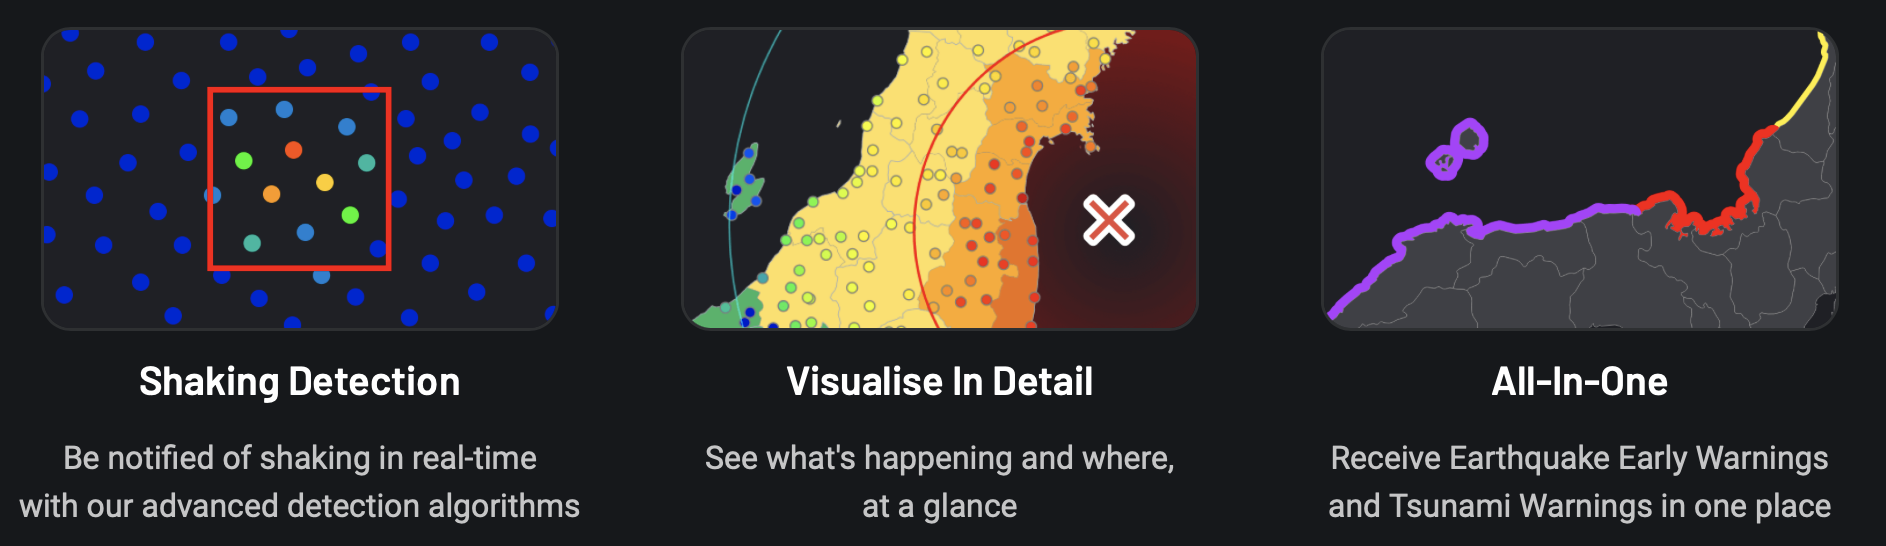
\includegraphics[width=0.6\linewidth]{jquake-features.png}
    \caption[Feature introduction of JQuake]{Feature introduction of JQuake, screenshot from website.}
    \label{fig:jquake-monitor-features}
\end{figure}

\begin{figure}[!ht]
    \centering

    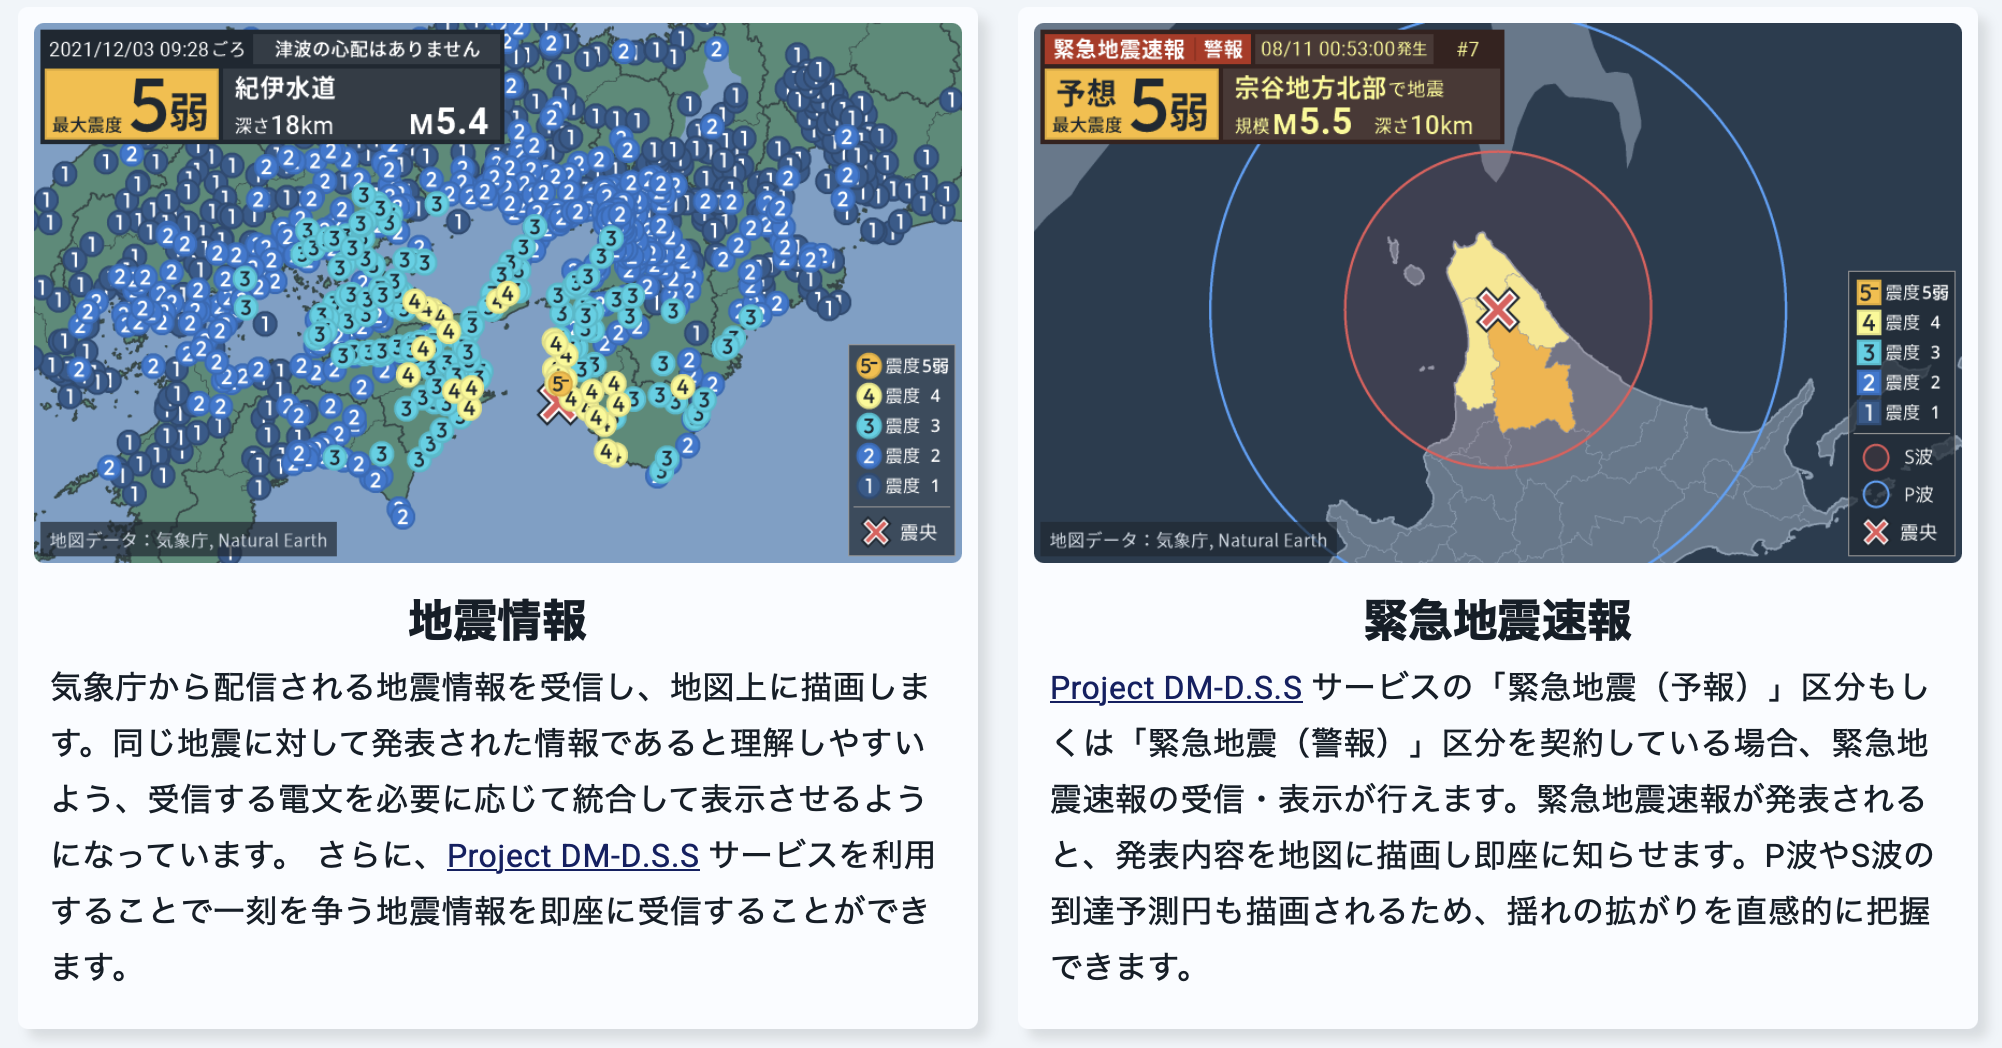
\includegraphics[width=0.6\linewidth]{quarog-features-1.png}\\
    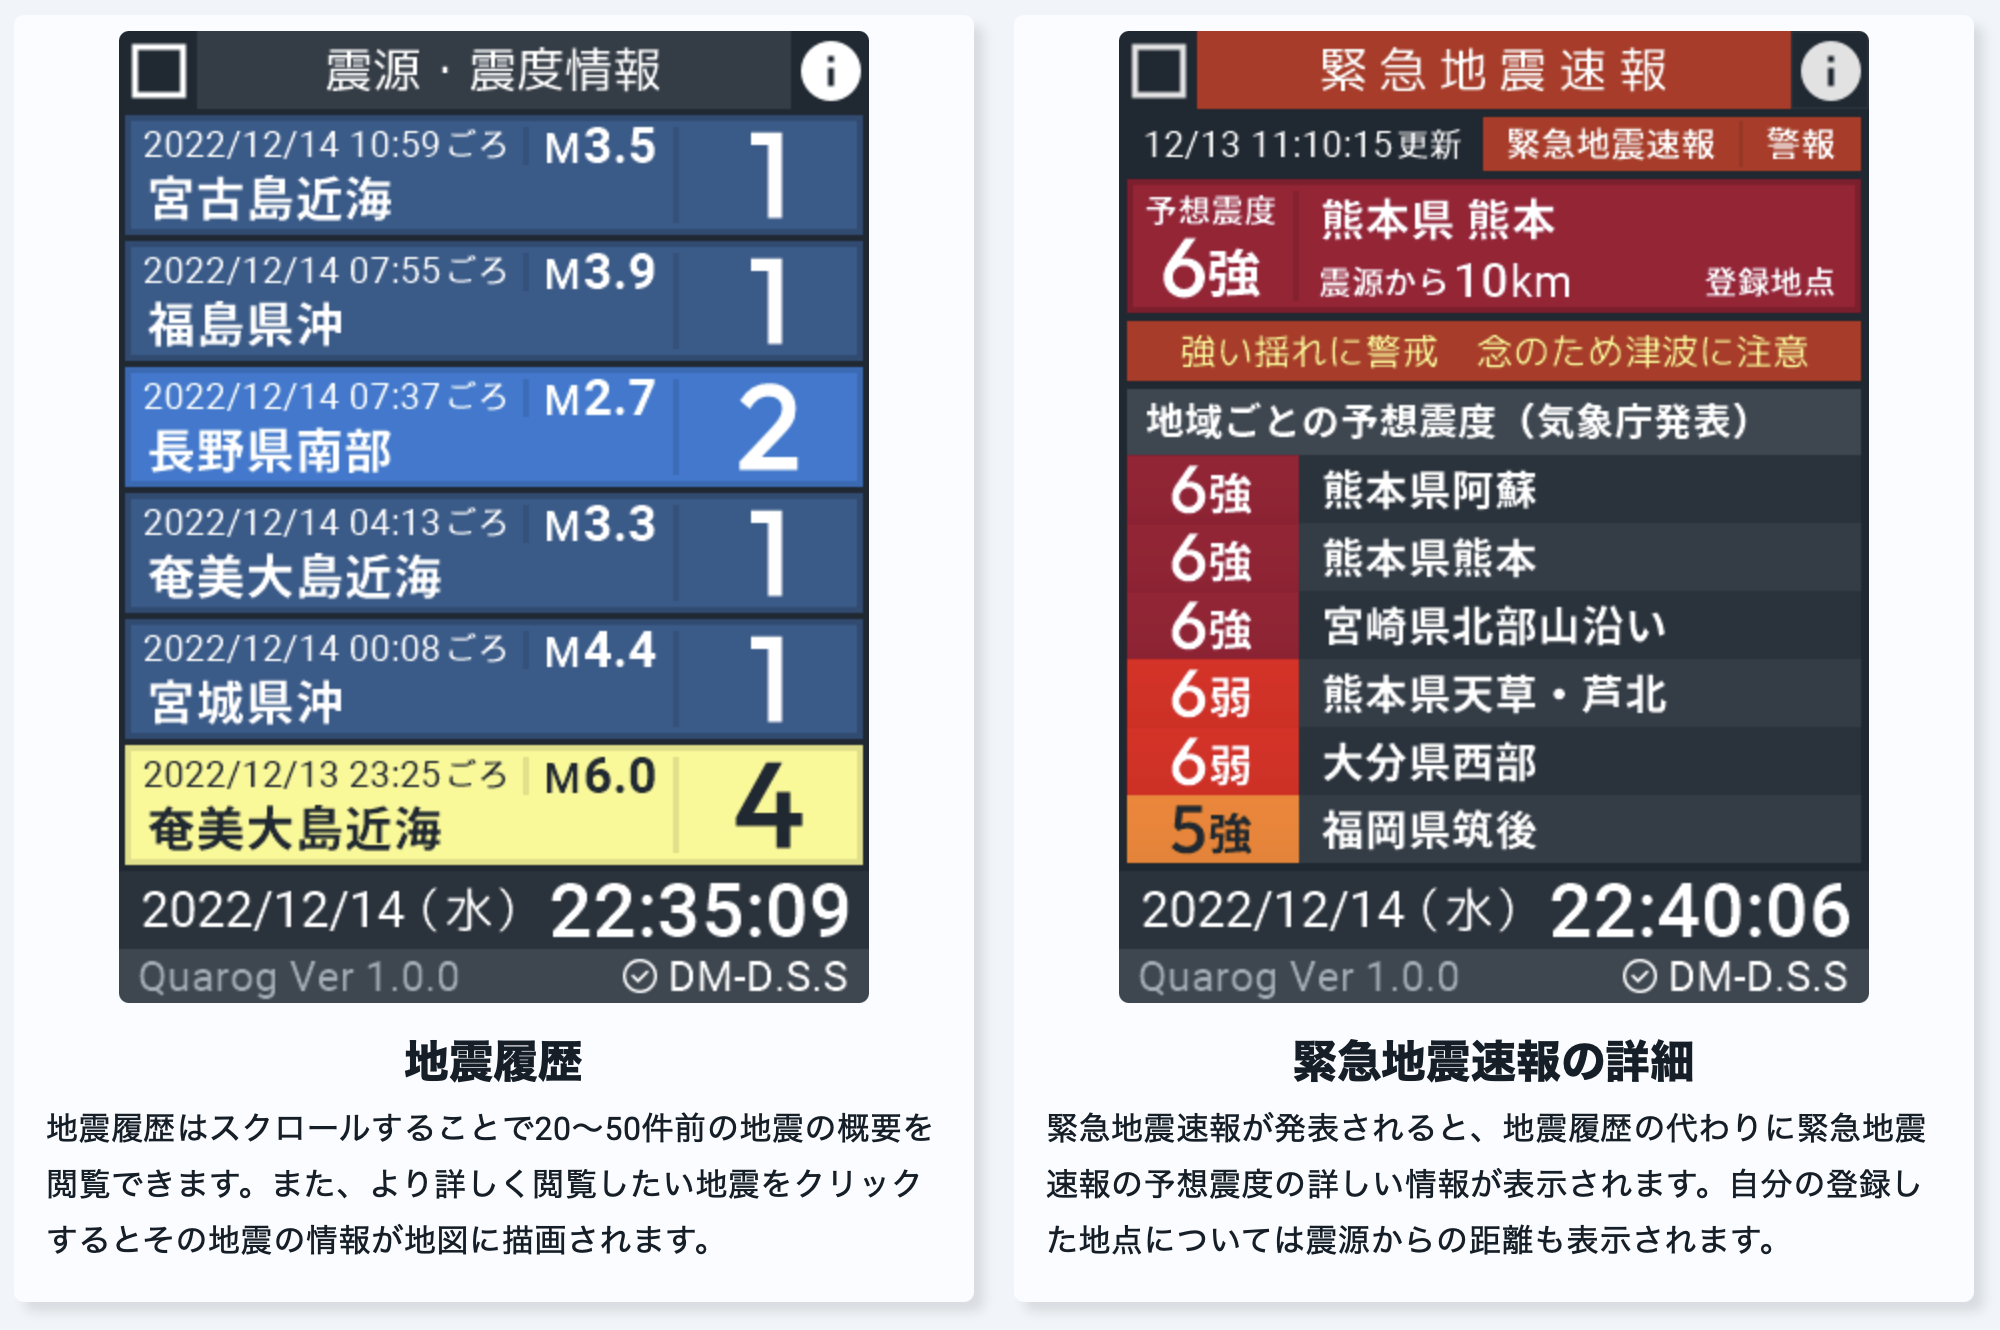
\includegraphics[width=0.6\linewidth]{quarog-features-2.png}
    \caption[Feature introduction of Quarog]{Feature introduction of Quarog, screenshot from website.\\Top-left: Past earthquake information; Top-right: Real-time EEW;\\Bottom-Left: Past earthquake list; Bottom-Right: Details of EEW.}
    \label{fig:quarog-monitor-features}
\end{figure}

There are also a variety of configuration options available for all apps, as listed in Table \ref{table:exist-config}. Both KEVI and Quarog supports the adjustment of the colour theme, and Quarog even supports changing the style of how blocks are displayed and coloured as shown in Figure \ref{fig:kevi-colour-cust} and \ref{fig:quarog-cust}. Playing a sound on the speaker is also common among the apps to remind the user of earthquakes.

\begin{table}[!ht]
    \centering

    \begin{tabular}{|c||c|c|c|c|}
        \hline
        Feature             & JQuake     & SREV       & KEVI       & Quarog     \\
        \hline
        DM-D.S.S. Login     & \checkmark &            & \checkmark & \checkmark \\
        Sound Alert         & \checkmark & \checkmark & \checkmark & \checkmark \\
        System Notification &            &            & \checkmark &            \\
        Colour Theme        &            &            & \checkmark & \checkmark \\
        Map Colouring Style &            & \checkmark &            & \checkmark \\
        \hline
    \end{tabular}
    \caption{Feature comparison in configuration and customisability of existing solutions}
    \label{table:exist-config}
\end{table}

\begin{figure}[!ht]
    \centering

    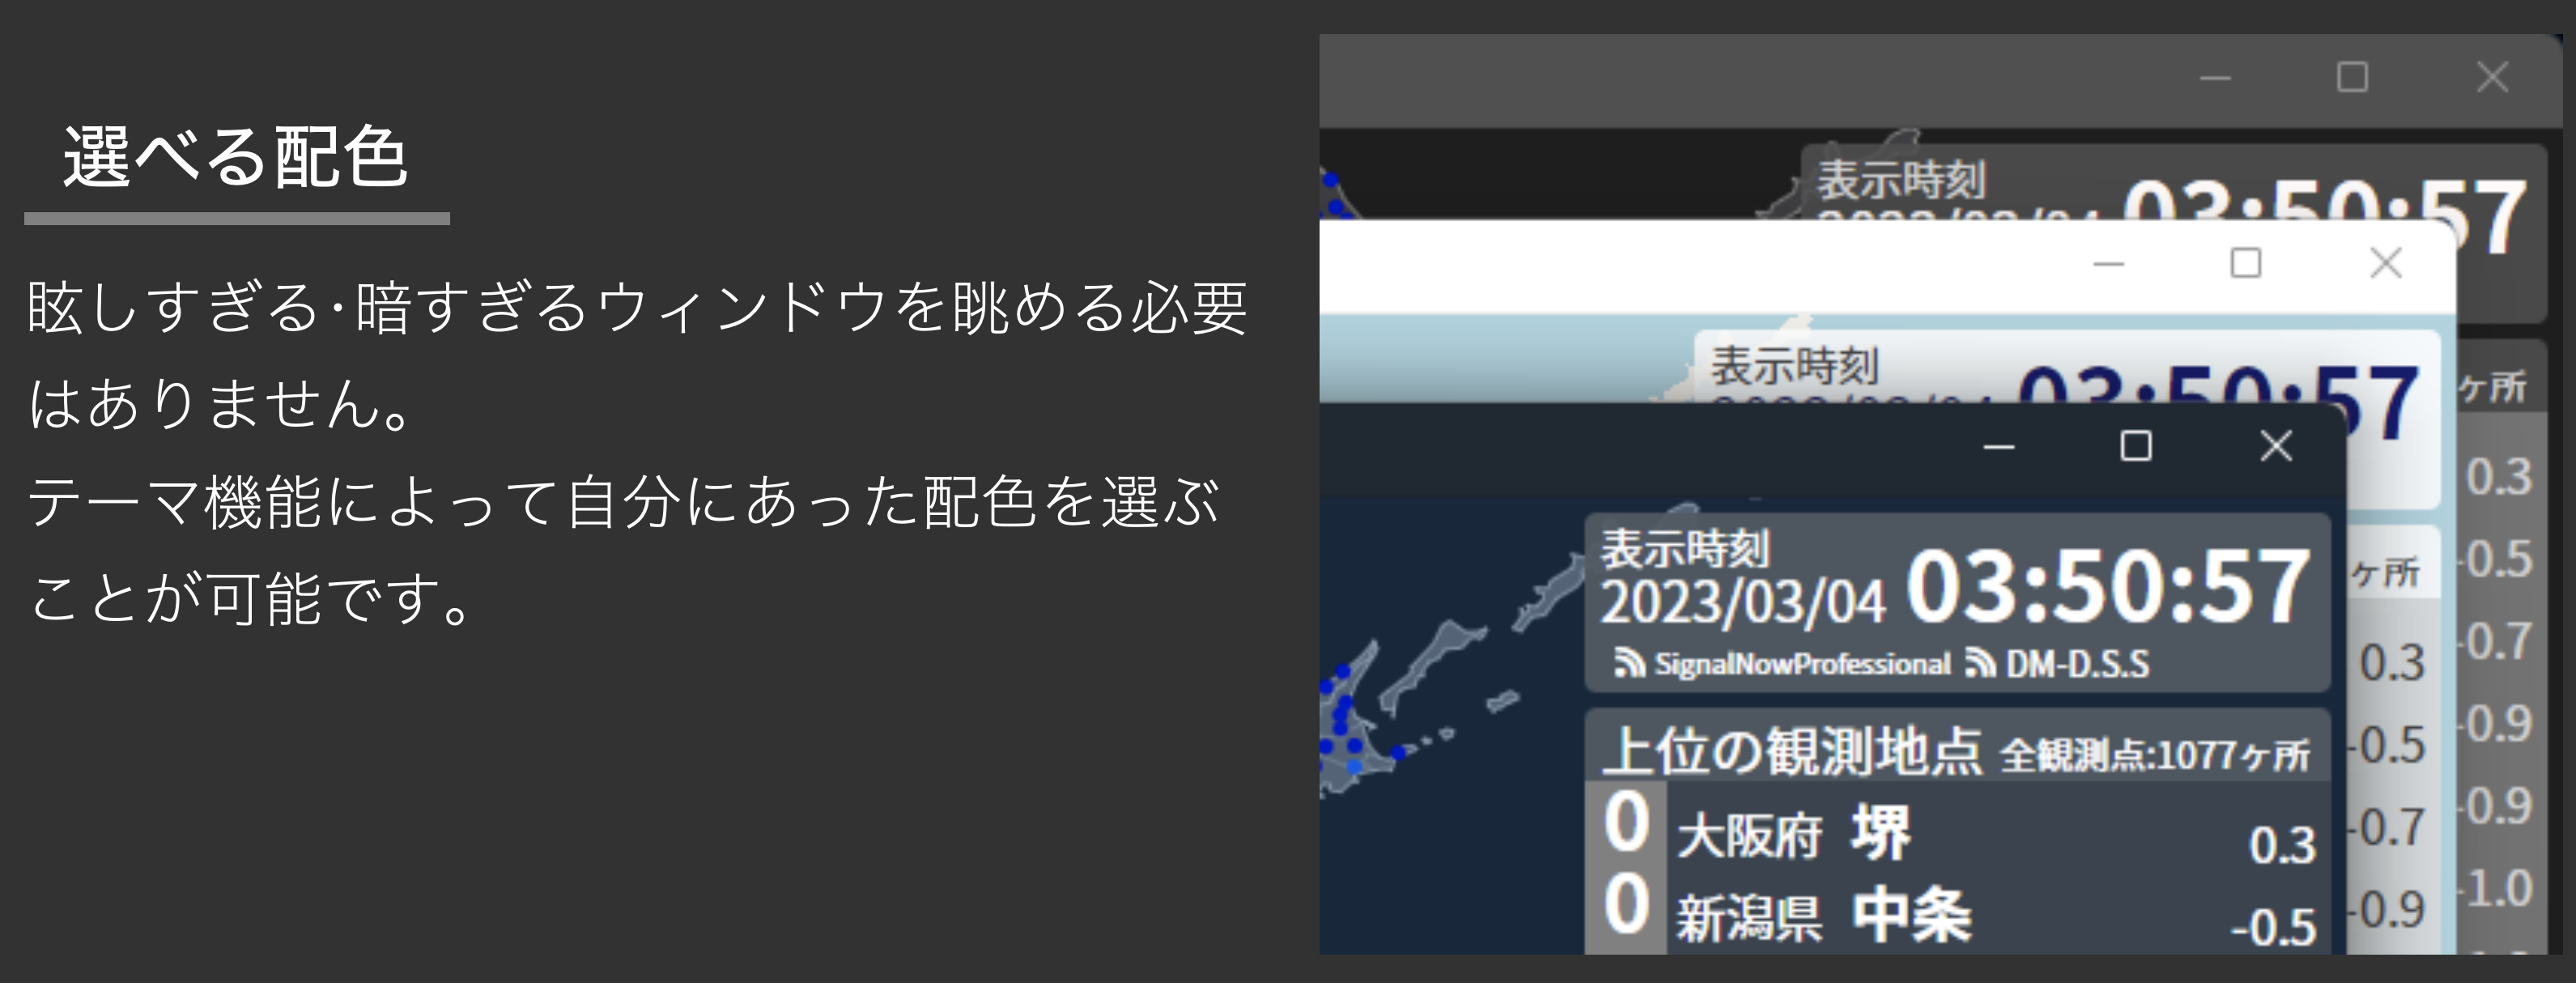
\includegraphics[width=0.5\linewidth]{kevi-colour.png}
    \caption[Customisable colour scheme of KEVI]{Customisable colour scheme of KEVI, screenshot from website.}
    \label{fig:kevi-colour-cust}
\end{figure}

\begin{figure}[!ht]
    \centering

    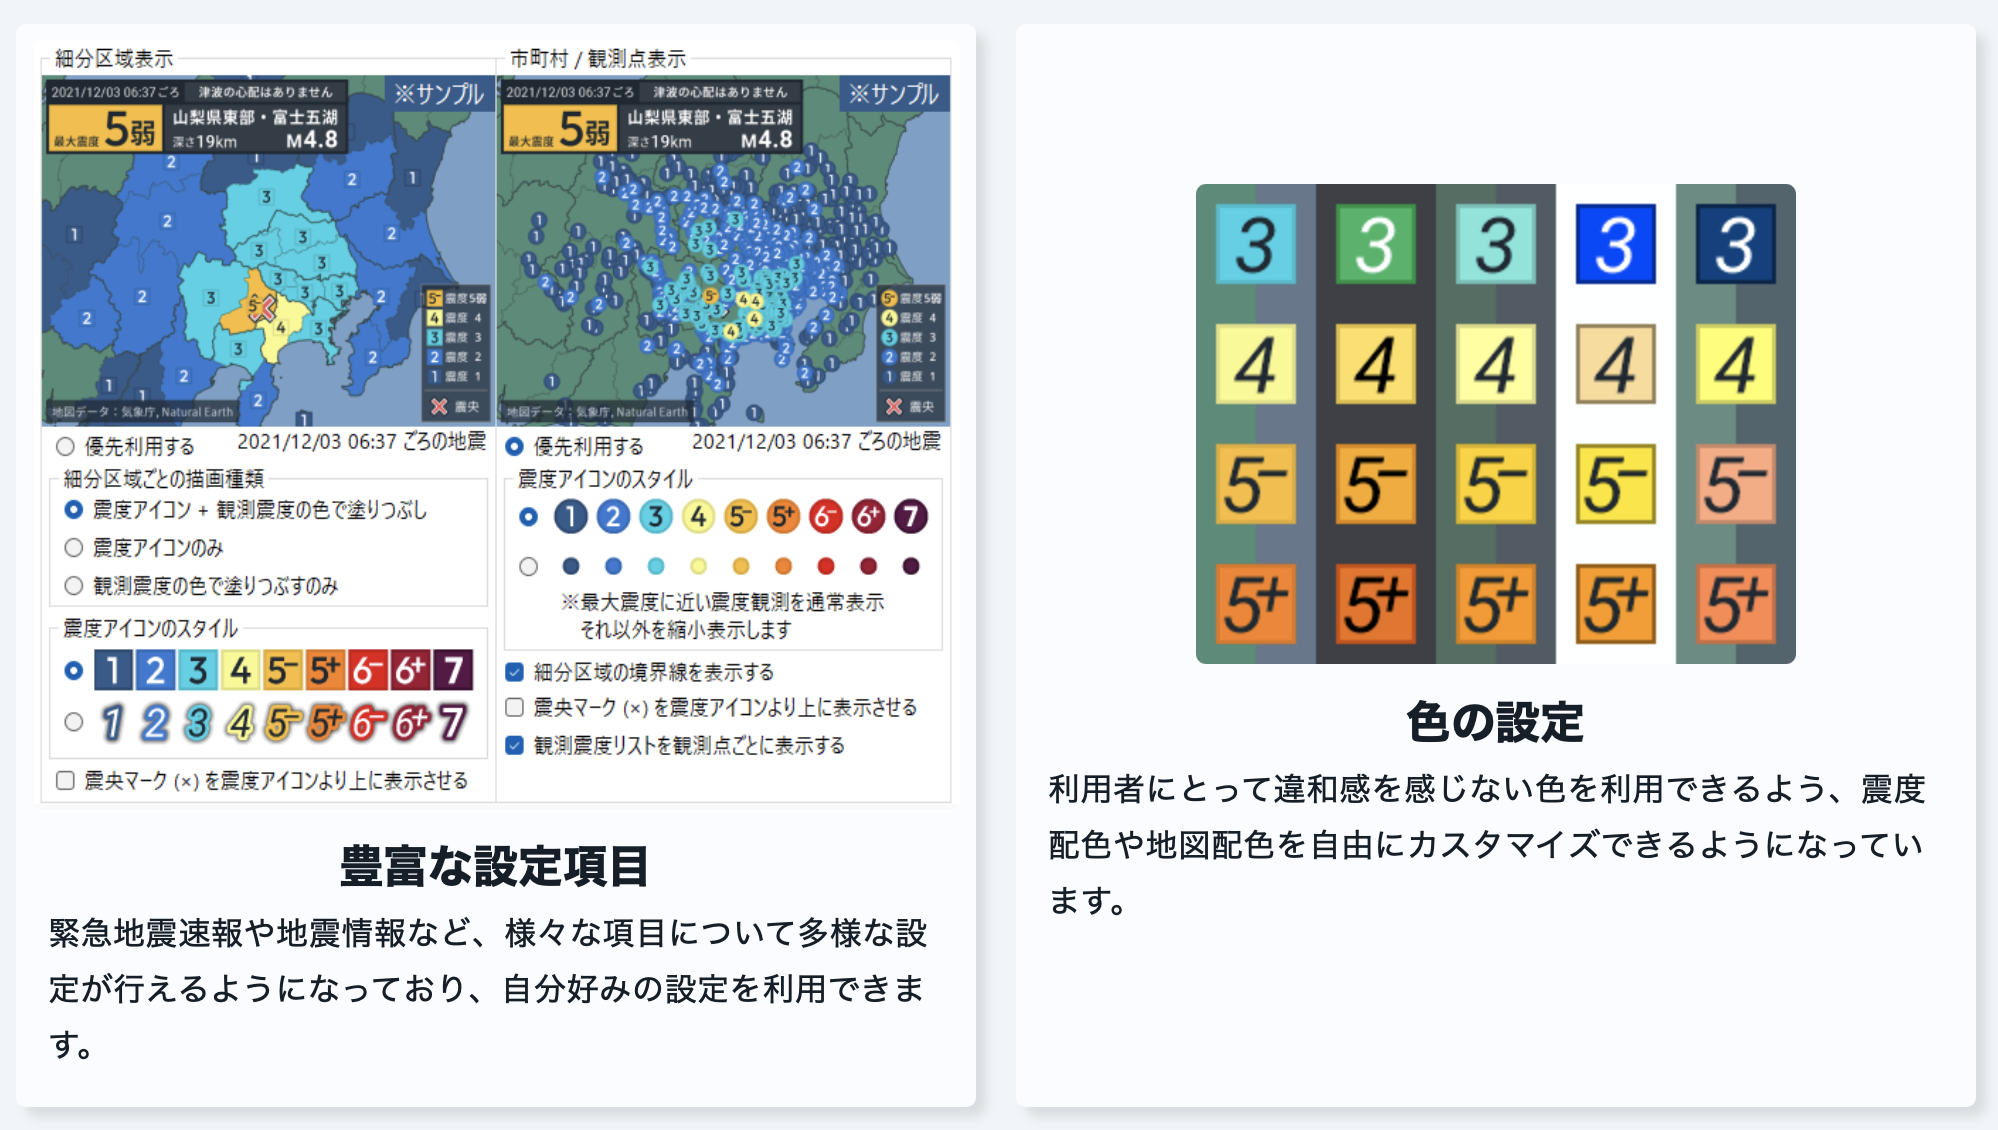
\includegraphics[width=0.6\linewidth]{quarog-cust.png}
    \caption[Customisability of Quarog]{Customisability of Quarog, screenshot from website.}
    \label{fig:quarog-cust}
\end{figure}

% TODO: Include analysis on GUI

\subsection{Features of proposed solution}

Based on the potential user/client interview results, and the research into the existing solutions, the following key features should appear in the solution, since they are essential to earthquake monitoring applications:
\begin{enumerate}
    \item DM-D.S.S. Login functionality (for the data source)
    \item Real-Time Sensor Shake Intensity Data (w/ vibration alert)
    \item EEW Visualisation (w/ Calculated Seismic Wavefronts)
    \item Past Earthquake List (w/ Option to review details)
    \item Tsunami Warning Visualisation (w/ Related Sounds)
\end{enumerate}

However, due to the limitation of time and the difficulty of implementation, the following functionalities are not the key to implementation, which include mostly the customisation parts, ranked in decreasing importance:
\begin{enumerate}
    \item User-Defined Key Monitor Point
    \item Customisable Sound Alert
    \item Customisable Colour Theme
    \item Customisable Map Colouring Style
\end{enumerate}

The following features might not be available due to the time constraints and the complexity behind such system:
\begin{enumerate}
    \item Replay (due to a server needing to store past data)
    \item Sub-Map for the Okinawa Area (due to the difficulty in implementation)
    \item Map Zooming Feature (due to the complexity in the map colouring functionality)
\end{enumerate}

With those key features implemented, the application should mirror all essential functionalities of an earthquake monitoring application, as compared to the four existing solutions above.

\subsection{Critical Path}

The functionality of this application can essentially be divided into \(1+2+1+n\) steps, where the 1 is to receive information from the API/WebSocket provided by DM-D.S.S. and NIED, and 2 is to, briefly saying:
\begin{enumerate}
    \item Real-time Monitoring: Produce a real-time map to monitor real time vibration and plot real-time EEW/tsunami warnings
    \item Past-earthquake Viewing: Produce a menu to select an earthquake to display information on the map.
\end{enumerate}

The next 1 is to merge these two functions, specifically the functionality to switch back to the real-time monitoring option immediately when a new EEW is released (to make sure the user does not miss any information on real-time EEWs while looking at past earthquake information).

The final \(n\) is to implement a setting page for customisation, and some extra additional features.

\bigskip

\paragraph{Part 1. NIED and DM-D.S.S. API/WebSocket Connection}
\begin{enumerate}
    \item Investigate into the list of APIs/WebSockets that should be used by the application.
    \item Implement classes/DTOs to convert the information into C\# objects.
    \item Implement classes to transfer real-time WebSocket XML/JSON to the classes and DTOs.
    \item Use simple API Key to test the functionality of this sub-system.
    \item Implement OAuth 2 login to reduce complexity and increase security.
\end{enumerate}

\paragraph{Part 2a. Real-time Monitoring Map}
\begin{enumerate}
    \item Implement a Japan map in the application.
    \item Achieve and store the locations of the monitoring points in Japan, using necessary information from JMA, NIED and DM-D.S.S.
    \item Colour the monitoring points using a colour scheme on the map.
    \item Investigate into and implement an algorithm to detect shake in a certain area of the map.
    \item Achieve and store the names of areas of earthquake epicentres from JMA.
    \item Investigate into and implement an algorithm to calculate seismic wave fronts.
    \item Plot and display real time EEWs, considering special cases such as:
          \begin{itemize}
              \item Cancellation of EEW;
              \item Upgrade from EEW Forecast to EEW Warning;
              \item Multiple Earthquakes (hence displaying epicentres with labels).
          \end{itemize}
    \item Implement functionality of colouring areas on the map with the maximum expected intensity.
    \item Achieve and store the names of shorelines from JMA.
    \item Plot and display real time tsunami warnings.
\end{enumerate}

\paragraph{Part 2b. Past-earthquake Viewing}
\begin{enumerate}
    \item Implement a side-list of a list of path earthquakes.
    \item Provide a button to view the detailed information on the earthquake (e.g. magnitude, epicentre, time).
    \item Implement functionality to plot the detected maximum intensities on the map, from where they are detected.
    \item Provide external link to view earthquake in the JMA website.
\end{enumerate}

\paragraph{Part 3. Joint functionality}
\begin{enumerate}
    \item Provide sidebar to switch between real-time monitoring and past-earthquake viewing.
    \item Implement automatic functionality to switch back to real-time earthquake monitoring when a shake over a certain magnitude is detected, or an EEW/Tsunami Warning is being published.
\end{enumerate}

\paragraph{Part 4. Setting page for customisation and some more}
\begin{enumerate}
    \item Implement customisable voice and sound playing (e.g. when EEW (over certain magnitude) is published, when an earthquake information detail is received, etc.)
    \item Implement customisable colour scheme for the colouring of different intensity scales, with several built in default.
    \item Implement key monitoring point with special warnings when an earthquake with more than a certain intensity is expected to hit that point.
    \item Implement a map-zooming feature.
    \item Implement a sub-map for the Okinawa Area.
\end{enumerate}

\subsection{Requirements Specification}

A detailed specification is defined here that is to be aimed to be fulfilled at the end of the project, split into four sections:
\begin{enumerate}
    \item \textbf{NIED and DM-D.S.S. Functionality} -- Corresponding to \textbf{Part 1}, in Table \ref{table:requirements-part-one}
    \item \textbf{Real-Time Earthquake Monitoring} -- Corresponding to \textbf{Part 2a}, in Table \ref{table:requirements-part-two-a}
    \item \textbf{Past-earthquake Viewing} -- Corresponding to \textbf{Part 2b}, in Table \ref{table:requirements-part-two-b}
    \item \textbf{GUI Design} -- Corresponding to \textbf{Part 3, 4}, in Table \ref{table:requirements-part-three}
\end{enumerate}

The objectives here are SMART, meaning they are specific, measurable, achievable, realistic and timely.

Note that those marked with an * means they are optional.

Table \ref{table:abbrs} for types of testing. [M] afterwards will stand for a necessary manual testing (i.e. specific user inputs), while (M) will stand for supplementary manual testing (i.e. will have stand-alone tests as well as manual tests).

\begin{table}[!ht]
    \centering
    \begin{tabular}{|c|c|}
        \hline
        Test Method         & Abbr. \\
        \hline
        Unit Testing        & UT    \\
        Integrated Testing  & IT    \\
        Performance Testing & PT    \\
        \hline
    \end{tabular}
    \caption{Measurement methods}
    \label{table:abbrs}
\end{table}

\begin{table}[!ht]
    \centering

    \begin{tabular}{|c||p{0.4\linewidth}|p{0.25\linewidth}|l|}
        \hline
        Req. \textnumero & Description                                              & Success Criteria                & Testing \\
        \hline \hline
        1(i)             & Login to DM-D.S.S. using an API Key                      & Login successful                & UT [M]  \\
        \hline
        1(ii)            & Call HTTP-Based APIs                                     & Successful calls                & UT (M)  \\
        \hline
        1(iii)           & Connect to WebSocket Data Feed                           & Successful calls                & UT [M]  \\
        \hline
        1(iv)            & Obtain stable connection on WS                           & Connected for 30min             & PT (M)  \\
        \hline
        1(v)             & Successfully parse JSON and XML into C\# objects         & Information successfully parsed & UT      \\
        \hline
        1(vi)            & Exception handling for incorrect JSON and XML            & Exceptions thrown               & UT      \\
        \hline
        1(vii)           & Exception handling for failed connections                & Exceptions thrown               & UT (M)  \\
        \hline
        1(viii)          & Integrated functionality from login to providing objects & Correct objects created         & IT [M]  \\
        \hline
        1(ix)*           & Login to DM-D.S.S. using OAuth2                          & Login successful                & UT (M)  \\
        \hline
    \end{tabular}
    \caption{Requirements for Part 1}
    \label{table:requirements-part-one}
\end{table}

\begin{table}[!ht]
    \centering

    \begin{tabular}{|c||p{0.4\linewidth}|p{0.25\linewidth}|l|}
        \hline
        Req. \textnumero & Description                                                                           & Success Criteria                                              & Testing    \\
        \hline \hline
        2a(i)            & Display real time shake-intensities on the map                                        & Correct coloured points at correct locations                  & IT         \\
        \hline
        2a(ii)           & Implement algorithm to display shake detection on the map                             & Use squares to indicate shake detected in area                & UT, IT, PT \\
        \hline
        2a(iii)          & Display the time at the corner of the UI                                              & Time displayed with less than 100ms error                     & UT         \\
        \hline
        2a(iv)           & Display real-time EEW when issued                                                     & Epicentre at correct position                                 & IT         \\
        \hline
        2a(v)            & Update/Cancel EEW when appropriate                                                    & Correctly updated and plotted                                 & IT         \\
        \hline
        2a(vi)           & Calculate and display seismic wavefronts by algorithm                                 & Calculated and plotted without significant delay              & UT, IT, PT \\
        \hline
        2a(vii)          & Colour map with expected maximum intensity of EEW                                     & Correctly coloured                                            & UT, IT     \\
        \hline
        2a(viii)         & Display the exp. magnitude, location, depth and intensity when EEW issued             & Correctly formatted and displayed                             & UT, IT     \\
        \hline
        2a(ix)           & Provide additional EEW information (e.g. detailed time, algorithm used) when prompted & Correctly formatted and displayed                             & IT [M]     \\
        \hline
        2a(x)            & Display tsunami warnings when issued                                                  & Coloured at correct location                                  & UT         \\
        \hline
        2a(xi)*          & Display real-time shake data at a user-defined point                                  & Display the name of the point with acceleration and intensity & IT         \\
        \hline
    \end{tabular}
    \caption{Requirements for Part 2(a)}
    \label{table:requirements-part-two-a}
\end{table}

\begin{table}[!ht]
    \centering

    \begin{tabular}{|c||p{0.4\linewidth}|p{0.25\linewidth}|l|}
        \hline
        Req. \textnumero & Description                                                                                             & Success Criteria                         & Testing \\
        \hline \hline
        2b(i)            & Display past-earthquake side list using data from DM-D.S.S.                                             & Displayed and updated                    & UT, IT  \\
        \hline
        2b(ii)           & Display the time, location, depth, intensity and magnitude of earthquake on the side list               & Correctly formatted and displayed        & UT, IT  \\
        \hline
        2b(iii)          & Colouring of the map by the maximum intensity of an earthquake when prompted                            & Correctly coloured                       & UT, IT  \\
        \hline
        2b(iv)           & Display details of shake and other additional information provided by JMA when prompted on a sub-window & Correctly formatted and displayed        & UT, IT  \\
        \hline
        2b(v)            & Provide link to external weather services for details                                                   & Linked to correct website and earthquake & UT [M]  \\
        \hline
        2b(vi)           & Provide link to JMA Earthquake details                                                                  & Linked to correct earthquake             & UT [M]  \\
        \hline
    \end{tabular}
    \caption{Requirements for Part 2(b)}
    \label{table:requirements-part-two-b}
\end{table}

\begin{table}[!ht]
    \centering

    \begin{tabular}{|c||p{0.4\linewidth}|p{0.3\linewidth}|l|}
        \hline
        Req. \textnumero & Description                                                               & Success Criteria                                     & Testing \\
        \hline \hline
        3(i)             & Provide sidebar to switch between real-time, past earthquake and settings & Sidebar functioning                                  & IT [M]  \\
        \hline
        3(ii)            & Switch to real-time monitoring map when EEWs are issued                   & Switch with delay less than 1s                       & IT, PT  \\
        \hline
        3(iii)           & Provide an easy-to-use GUI                                                & Potential user gives rating of more than 7 out of 10 & [M]     \\
        \hline
        3(iv)*           & Provide page to design custom colour scheme                               & Colour scheme designed and applied to the whole UI   & UT      \\
        \hline
        3(v)*            & Play sound when events happen and provide option to customise sound files & Correct sound played when required                   & UT, IT  \\
        \hline
        3(vi)*           & Provide option to define a point on the map to monitor                    & Option provided and meet specs defined in Part 2a    & UT, IT  \\
        \hline
        3(vii)*          & Provide zooming feature on map                                            & Map functioning with specs in Part 2                 & UT, IT  \\
        \hline
        3(viii)*         & Provide sub-map to display Okinawa Area                                   & Map functioning with specs in Part 2                 & UT, IT  \\
        \hline
    \end{tabular}
    \caption{Requirements for Part 3}
    \label{table:requirements-part-three}
\end{table}

\section{Design}
\subsection*{Overview}
This section includes a breakdown of the application into sections of data processing, GUI functionalities and joint functionalities. The use of external sources including DM-D.S.S. and NIED data sources is discussed, together with the relevant formats (XML, JSON) and the objects related. A UML class diagram is included to discuss OOP relations of classes, records (record classes) and enums including use of inheritance, composition, association and aggregation. They also implement different interfaces. An outline of the design of the user interface is included. The expected hardware requirements of the systems are also listed, but any laptop with an up-to-date operating system (running Windows or macOS) should be able to run the program.

\subsection{Data Structures/Data modelling}

\subsubsection{External Data Sources}
There are two data sources this program will use: the NIED and the DM-D.S.S. Specifically, the former one is used to achieve the real-time shake data of the sensor points which were set up by the government (whose data is free to use), and the latter one is used to achieve past earthquake information and EEW information sent out by the JMA (which is pay-to-use). Note that DM-D.S.S. does also provide the real-time intensity data of the observation points, however it is pay-to-use only for companies and institutions on request. Therefore, it will not be feasible to use this data source in the program since one of and the principle target users is people passionate in monitoring earthquakes.

\paragraph{NIED Data Source}

As mentioned before, NIED has numerous 'earthquake observation nets' across Japan. Specifically, there is the \href{https://www.kyoshin.bosai.go.jp/kyoshin/}{K-NET and the KiK-net}, which is dedicated to the observation of strong seismic motion. The K-NET consists of approximately 1000 sensors located across Japan, while the KiK-net also includes some sensors which are located within the earth, which will often have different readings compared to those located on the surface. They are extremely capable of detecting strong motion of ground. Furthermore, the K-NET and the KiK-net provides real-time intensity data webpage of two types, the \href{http://www.kmoni.bosai.go.jp}{'Kyoshin' monitor} and the \href{https://www.lmoni.bosai.go.jp/monitor/}{long-period ground motion (LPGM) monitor (not working at the time of investigation)}. The \href{https://www.hinet.bosai.go.jp/?LANG=ja}{Hi-net} stands for high-sensitivity seismograph network, and it is dedicated for observation of minor motions of the ground. They release the waveforms to those who are researching seismic movements. As for the \href{https://www.fnet.bosai.go.jp/freesia/top.php?LANG=ja}{F-net} which stands for the Full Range Seismograph Network of Japan, which is used to analyse the mechanism of a certain earthquake by analysing movements. None of the three nets provide a real-time API data feed.

Having compared the functionalities described above of the K/KiK-net, Hi-net and F-net and how they feed the data sources, the most suitable data source to reflect real-time motion of ground movements will be the \textbf{K/KiK-net}'s data feed, since it detects strong ground movements and is available real-time for the purpose of the application. (This is also the data source that JQuake and KEVI use in fact.)

In fact, in addition to these three networks, there are also the S-net, the DONET and the N-net, which detects the ground seismic movements in the sea. These data were adapted by SREV, but this is beyond the scope of this NEA analysis.

A comparison from the official website of \href{https://www.mowlas.bosai.go.jp}{MOWLAS (Monitoring of Waves on Land and Seafloor)} of the three nets are included in Figure \ref{fig:net-comparison} and a map of the distribution of the sensors are included in Figure \ref{fig:net-distribution}.

\begin{figure}[!ht]
    \centering
    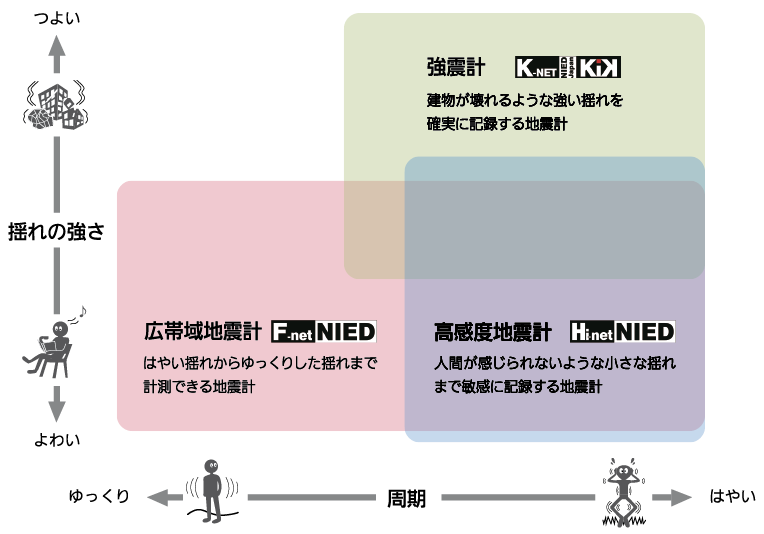
\includegraphics[width = 0.75\linewidth]{net-comparison.png}
    \caption{A comparison of the K-NET, F-net and Hi-net.}
    \label{fig:net-comparison}
\end{figure}

\begin{figure}[!ht]
    \centering
    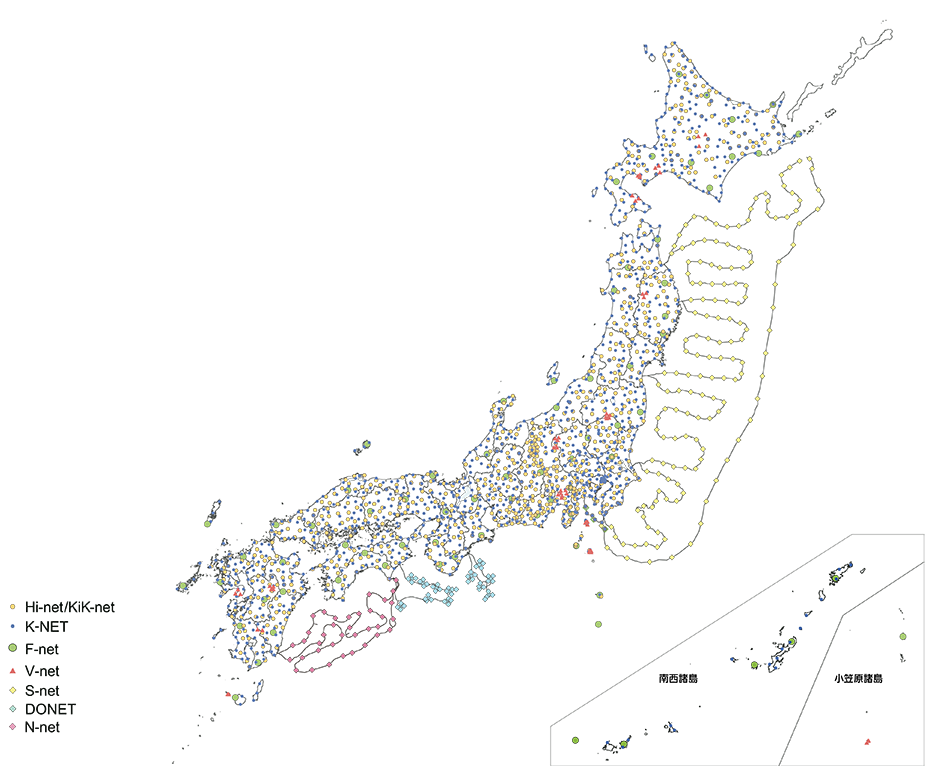
\includegraphics[width = 0.75\linewidth]{net-distribution.png}
    \caption{Distribution of the sensors of different nets.}
    \label{fig:net-distribution}
\end{figure}

% TODO: Citation

\subparagraph{Achieving image format data source}

The data source fed by the 'Kyoshin' Monitor is split into 8 types (detailed below in Table \ref{table:kmoni-data-types}), and each type split into 2 types of data sources, surface sensors and borehole (earth) sensors, with codes in Table \ref{table:kmoni-sensor-types}. The link to the GIF image is in the following format:

\begin{center}
    \url{http://www.kmoni.bosai.go.jp/data/map_img/RealTimeImg/[#1]_[#2]/[yyyyMMdd]/[yyyyMMdd][hhmmss].[#1]_[#2].gif}
\end{center}

In the link, the [yyyyMMdd] and the [hhmmss] part should be replaced with the date and time respectively (in JST, UTC+8), and the \#1 replaced with the codes detailed below for the data types, and \#2 replaced with the codes detailed below for data sources. An example of the imaged achieved is in Figure \ref{fig:sample-kmoni}

\begin{table}[!ht]
    \centering

    \begin{tabular}{|c|c|c|}
        \hline
        Data Type        & Description/Meaning                & Code in \@1 \\
        \hline
        Real-time Shindo & Real-time Measured Intensity       & jma         \\
        PGA              & Peak (Maximal) Ground Acceleration & acmap       \\
        PGV              & Peak (Maximal) Ground Velocity     & vcmap       \\
        PGD              & Peak (Maximal) Ground Displacement & dcmap       \\
        Response 0.125Hz & Response spectrum for 0.125Hz PGV  & rsp0125     \\
        Response 0.250Hz & Response spectrum for 0.250Hz PGV  & rsp0250     \\
        Response 0.500Hz & Response spectrum for 0.500Hz PGV  & rsp0500     \\
        Response 1.000Hz & Response spectrum for 1.000Hz PGV  & rsp1000     \\
        Response 2.000Hz & Response spectrum for 2.000Hz PGV  & rsp2000     \\
        Response 4.000Hz & Response spectrum for 4.000Hz PGV  & rsp4000     \\
        \hline
    \end{tabular}
    \caption{Data available in 'Kyoshin' monitor}
    \label{table:kmoni-data-types}
\end{table}

\begin{table}[!ht]
    \centering

    \begin{tabular}{|c|c|c|}
        \hline
        Sensor Type & Description/Meaning          & Code in \@1 \\
        \hline
        Surface     & K-NET and KiK-net sensors    & s           \\
        Borehole    & KiK-net sensors within earth & b           \\
        \hline
    \end{tabular}
    \caption{Sensors available in 'Kyoshin' monitor}
    \label{table:kmoni-sensor-types}
\end{table}

\begin{figure}[!ht]
    \centering
    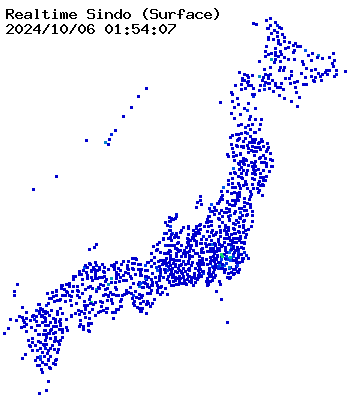
\includegraphics[width = 0.5\linewidth]{sample-kmoni.png}
    \caption{Sample GIF image achieved from 'Kyoshin' Monitor}
    \label{fig:sample-kmoni}
\end{figure}

\subparagraph{Extracting colour for each observation point from image}

Unfortunately, it seems to the author (and is widely accepted in the EEW monitoring app development society) that the position of the points (squares) on the image does not follow any significant pattern of position, i.e. there is no obvious conversion of coordinates to us from the official longitude/latitude locations to the positions on the image. Therefore, a manual conversion one-to-one mapping has to be developed.

NIED does have an official released list of observation points, which include their names and positions. This list has around 1700 of those observation points. However, in the actual image (like those in Figure \ref{fig:sample-kmoni}), there are only 1000 of those in use in real time, consistent with K-NET's official introduction, and the rest 700 of those are invalid observation points. Therefore, it will be worth removing them from the list of earthquake monitoring points, before attempting to make the dictionary.

Unfortunately, 1000 is still quite a lot for us to deal with. Luckily, Ingen who used a similar approach to develop the KEVI application has already made such a mapping inside his open-source application in the file \href{https://github.com/ingen084/KyoshinEewViewerIngen/blob/develop/src/KyoshinEewViewer/Assets/ShindoObsPoints.mpk.lz4}{ShindoObsPoints.mpk.lz4} within \GitHubHref{ingen084}{KyoshinEewViewerIngen}, and even developed an editor for this at \GitHubHref{ingen084}{KyoshinShindoPlaceEditor}.

Due to the limited time for this NEA, the author will primarily use the pre-determined observation points for the K-net, and will use the existing application to map the points for KiK-net, which is still a considerable amount of work, but significantly less.

This paragraph referred to \href{https://qiita.com/ingen084/items/7e91f8da2996972ac586}{this blog article} written by Ingen.

% TODO: Where is the list?

\subparagraph{Converting colour back to number format for further processing}

The true numerical data does not seem fully necessary at the first glance (since we might just as well just achieve the colour from the image and just plot them on the map, without the need to convert to a colour and back). However, for us to detect the shake in certain regions, it is necessary for us to achieve the numerical value to run the algorithm on it. Nevertheless, it is just good to have the number for us to have the numerical value for potential future developments.

\begin{figure}[!ht]
    \centering
    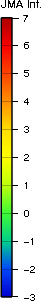
\includegraphics[scale = 0.6]{jma-scale.png}
    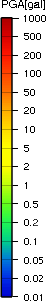
\includegraphics[scale = 0.6]{pga-scale.png}
    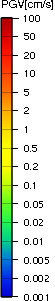
\includegraphics[scale = 0.6]{pgv-scale.png}
    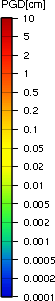
\includegraphics[scale = 0.6]{pgd-scale.png}
    \caption{Scale colours of different measurements}
    \label{fig:scale-colour}
\end{figure}

As shown in Figure \ref{fig:scale-colour}, the NIED 'Kyoshin' Monitor does indeed provide a scale of colours and reference to numerical values. However, there is a chance that a certain colour is not 'exactly' mapped on the scale, and further concerning that it is very slow and difficult to 'loop over' a colour legend, it is necessary to have an algorithmic-approach (numerical mapping-based approach) to map the colours in the colour space to numerical values (and back) is necessary.

Notice that the scale for PGA/PGV/PGD follow a logarithmic scale, while measured intensity follows a linear scale (though noting that the way intensity and magnitude is calculated is logarithmic as well). Therefore, if we normalise the vertical distance from the bottom of the axis \(h\) to \(0 \leq h \leq 1\) (i.e. \(h = 0\) at the bottom of the scale, \(h = 1\) at the top of the scale), and if we denote intensity using \(I\) in JMA scale, PGA as \(a\) in gal, PGV as \(v\) in cm per second, and PGD as \(s\) in cm, from the scale, the following transforming formulae obviously hold:
\begin{align*}
    I  = 10h - 3     & \iff h      = \frac{I + 3}{10}, \\
    a  = 10^{5h - 2} & \iff h  = \frac{\lg a + 2}{5},  \\
    v  = 10^{5h - 3} & \iff h  = \frac{\lg v + 3}{5},  \\
    x  = 10^{5h - 4} & \iff h  = \frac{\lg x + 4}{5}.  \\
\end{align*}

However, it is worth noting that NIED did use \(1, 2, 5, 10\) on the logarithmic scale at equal intervals, so it is not a perfect logarithmic scale. The author is unsure why they designed the scale like this, nor if it's an intended approximation. Nevertheless, the logarithmic scale is a good enough approximation.

The next step is to develop a mapping from this colour space \(\mathcal{C}\) to \(h\), which of course should be invertible. Denote this as \(f: [0, 1] \to \mathcal{C}\).

We consider using a suitable base to decompose \(\mathcal{C}\). The colour of the given scale is an immediate suggestion to use a base containing \textbf{hue}, which in fact is designed to describe how human perceive colour, and unlike RGB and CMYK which uses principle colours to describe colour. A hue scale is shown in Figure \ref{fig:hue-scale}.

\begin{figure}[!ht]
    \centering
    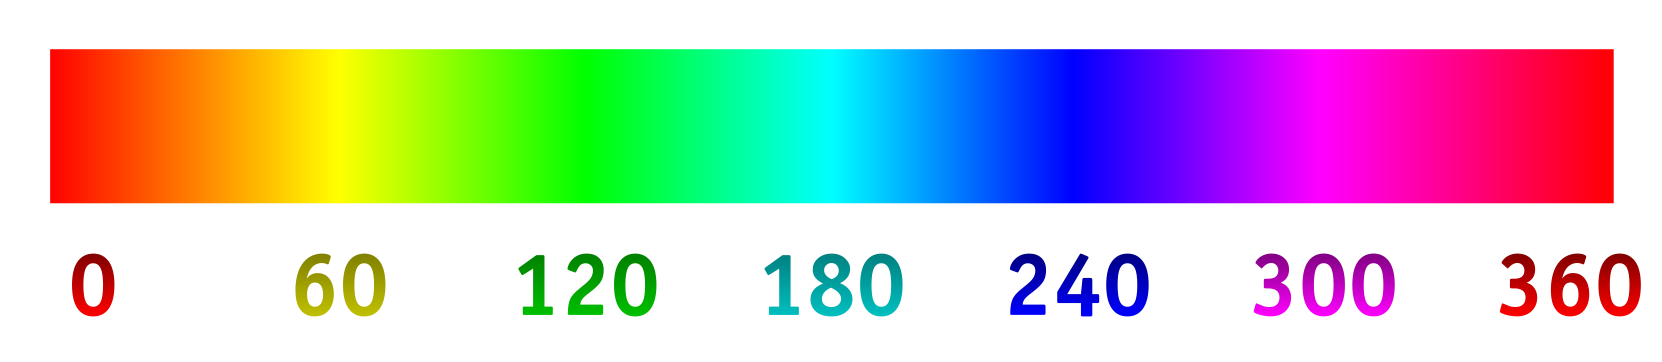
\includegraphics[scale = 0.15]{hue-scale.png}
    \caption{The hue scale in HSL/HSV encoding}
    \label{fig:hue-scale}
\end{figure}

Therefore, a colour in the colour space \(\mathcal{C}\) can be represented as a 3-D vector \(\mathcal{C} \ni C = (H, S, V)\), where \(H \in [0, 360)\) in degrees is the hue value, \(S \in [0, 1]\) stands for the saturation, and \(V \in [0, 1]\) stands for the value (a brightness). And hence we will be able to decompose \(f\) into three components \(f = \left(f_H, f_S, f_V\right)\).

Figure \ref{fig:hsv-against-row} plots the values of \(H, S\) and \(V\) against \(h\) (this is the graph of \(f\) and its components) of discrete values of \(h\), and depending on the result we will attempt some fit/regression to a suitable function.

\begin{figure}[!ht]
    \centering
    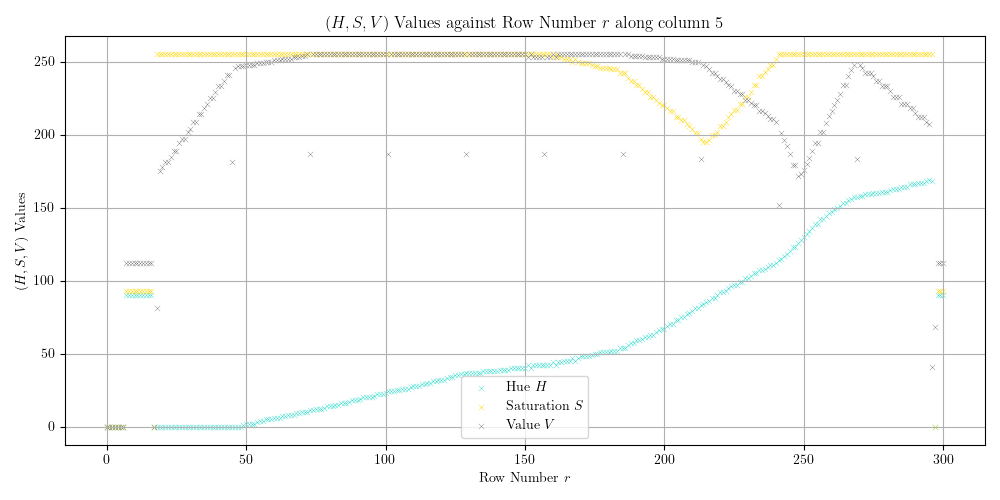
\includegraphics[scale = 0.55]{hsv-against-row.png}
    \caption{The values of \((H, S, V)\) against pixel row \(r\)}
    \label{fig:hsv-against-row}
\end{figure}

Notice that in this plot, all values of \((H, S, V)\) in fact range from \(0\) to \(255\).

It is worth noting that the scale has some space on the top (to show the type), and some space at the bottom. Notice that when the row \(r = 17\) and \(r = 297\) have values significantly different, so we extract the rows \(r = 18\) and \(r = 296\) to correspond (linearly) to \(h = 1\) and \(h = 0\), i.e.,
\[
    h = 1 - \frac{r - 18}{278}.
\]

Figure \ref{fig:hsv-against-h} shows the result of this transformation being applied.

\begin{figure}[!ht]
    \centering
    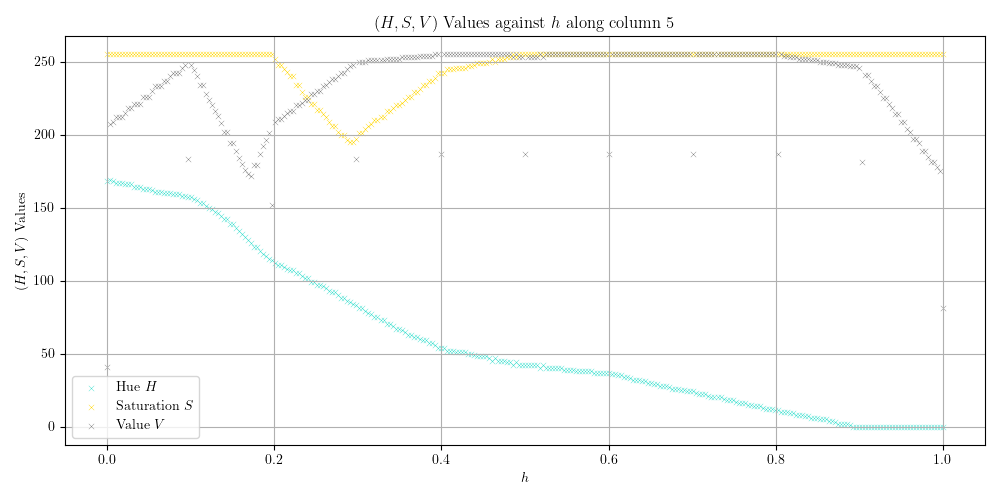
\includegraphics[scale = 0.55]{hsv-against-h.png}
    \caption{The values of \((H, S, V)\) against normalised height \(h\)}
    \label{fig:hsv-against-h}
\end{figure}

From here onwards, all values of \((H, S, V)\) will be adjusted to be within the range which they should be in, i.e. \(H \in [0, 360), S \in [0, 1], V \in [0, 1]\).

We consider finding \(f_H\) first, which is the cyan line. Notice that its trend can be split into 4 parts:
\begin{itemize}
    \item \(h \in [0, 0.1]\): linear;
    \item \(h \in [0.1, 0.6]\): curving, ideally a cubic;
    \item \(h \in [0.6, 0.9]\): linear;
    \item \(h \in [0.9, 1]\): constant (0).
\end{itemize}

\begin{table}[!ht]
    \centering

    \begin{tabular}{|c|c|}
        \hline
        \(h\) & \(H = f_H(h)\) \\
        \hline
        0     & 237            \\
        0.1   & 222            \\
        0.6   & 51             \\
        0.9   & 0              \\
        1     & 0              \\
        \hline
    \end{tabular}
    \caption{Initial values for \(f_H\)}
    \label{table:h-against-h-iv}
\end{table}

Furthermore, boundary conditions in Table \ref{table:h-against-h-iv} are applied to ensure that the function is continuous and nicely-behaving while matching the existing data. We use the following function to apply the fit:
\[
    f_H(h) = \begin{cases}
        -150h + 237, & h \in [0, 0.1],   \\
        \odot,       & h \in [0.1, 0.6], \\
        -170h + 153, & h \in [0.6, 0.9], \\
        0,           & h \in [0.9, 1].
    \end{cases}
\]

Here,
\begin{align*}
    \odot & = \frac{222 \cdot (h - 0.3) \cdot (h - 0.4) \cdot (h - 0.6)}{(0.1 - 0.3) \cdot (0.1 - 0.4) \cdot (0.1 - 0.6)} \\
          & + \frac{y_1 \cdot (h - 0.1) \cdot (h - 0.4) \cdot (h - 0.6)}{(0.3 - 0.1) \cdot (0.3 - 0.4) \cdot (0.3 - 0.6)} \\
          & + \frac{y_2 \cdot (h - 0.1) \cdot (h - 0.3) \cdot (h - 0.6)}{(0.4 - 0.1) \cdot (0.4 - 0.3) \cdot (0.4 - 0.6)} \\
          & + \frac{51 \cdot (h - 0.1) \cdot (h - 0.3) \cdot (h - 0.4)}{(0.6 - 0.1) \cdot (0.6 - 0.3) \cdot (0.6 - 0.4)}.
\end{align*}

Here, \(m_1\) is the gradient of the line for \(h \in [0, 0.1]\), \(y_1 = f_H(0.3), y_2 = f_H(0.4)\) for \(h \in [0.1, 0.6]\) (using Lagrange Polynomial), and the equation between \(h \in [0.6, 0.9]\) is in fact fixed due to the initial conditions.

By applying a curve fit to the original data, the following results are obtained:
\[
    (y_1, y_2) = (115, 79.5).
\]

Plotting \(H\) and \(f_H(h)\) against \(h\) gives us Figure \ref{fig:h-against-h}, which is decent.

\begin{figure}[!ht]
    \centering
    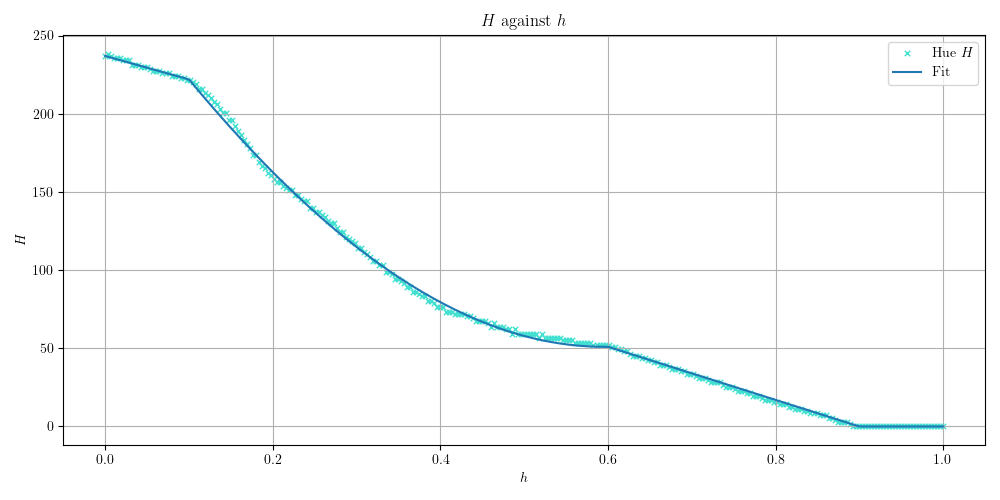
\includegraphics[scale = 0.55]{h-against-h.png}
    \caption{The fit result for \(f_H: h \mapsto H\)}
    \label{fig:h-against-h}
\end{figure}

As for \(f_S(h)\), the obvious thing to do is to split it into 5 (4) piecewise functions, specifically \(f_S = 1\) for \(h \in [0, 0.2] \cup [0.5, 1]\), and three linear functions for \(h \in [0.2, 0.29], h \in [0.29, 0.4]\) and \(h \in [0.4, 0.5]\). Initial values are included in Table \ref{table:s-against-h-iv}.

\begin{table}[!ht]
    \centering

    \begin{tabular}{|c|c|}
        \hline
        \(h\) & \(S = f_S(h)\) \\
        \hline
        0     & 1              \\
        0.2   & 1              \\
        0.29  & 0.765          \\
        0.4   & 0.95           \\
        0.5   & 1              \\
        1     & 1              \\
        \hline
    \end{tabular}
    \caption{Initial values for \(f_S\)}
    \label{table:s-against-h-iv}
\end{table}

This gives us that
\[
    f_S(h) = \begin{cases}
        1,              & h \in [0, 0.2],    \\
        -2.611h + 1.522 & h \in [0.2, 0.29], \\
        1.682h + 0.277, & h \in [0.29, 0.4], \\
        0.5h + 0.75     & h \in [0.4, 0.5],  \\
        1,              & h \in [0.5, 1].
    \end{cases}
\]

Plotting this out gives Figure \ref{fig:s-against-h}.

\begin{figure}[!ht]
    \centering
    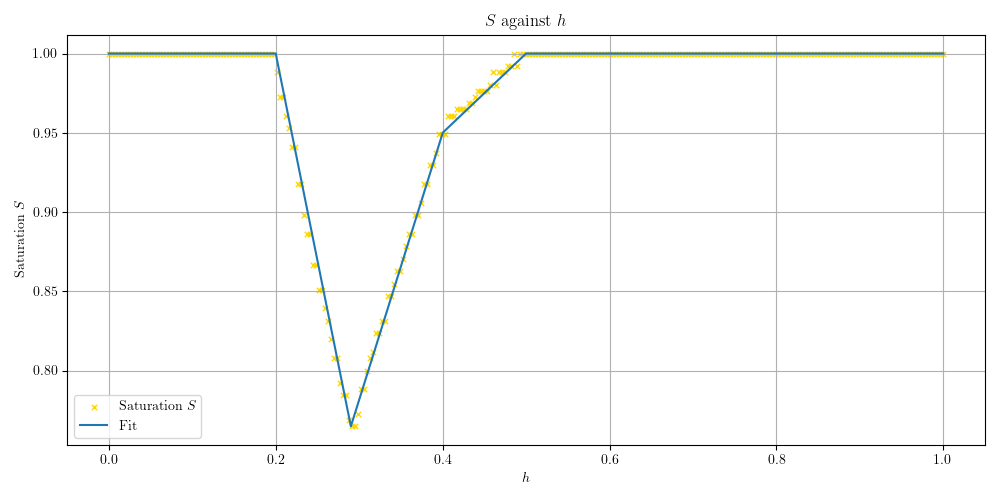
\includegraphics[scale = 0.55]{s-against-h.png}
    \caption{The fit result for \(f_S: h \mapsto S\)}
    \label{fig:s-against-h}
\end{figure}

As for \(f_V(h)\), we shall divide it into even more piecewise linear functions. Specifically, I chose the intervals \([0, 0.1], [0.1, 0.175], [0.175, 0.2], [0.2, 0.3], [0.3, 0.4], [0.4, 0.8], [0.8, 0.9]\) and \([0.9, 1]\). Initial values are included in Table \ref{table:v-against-h-iv}.

\begin{table}[!ht]
    \centering

    \begin{tabular}{|c|c|}
        \hline
        \(h\) & \(V = f_V(h)\) \\
        \hline
        0     & 0.8            \\
        0.1   & 0.98           \\
        0.172 & 0.66           \\
        0.2   & 0.82           \\
        0.3   & 0.98           \\
        0.4   & 1              \\
        0.8   & 1              \\
        0.9   & 0.97           \\
        1     & 0.68           \\
        \hline
    \end{tabular}
    \caption{Initial values for \(f_V\)}
    \label{table:v-against-h-iv}
\end{table}

This gives us the piecewise function
\[
    f_V(h) = \begin{cases}
        1.8h + 0.8,      & h \in [0, 0.1],     \\
        -4.444h + 1.424, & h \in [0.1, 0.172], \\
        5.714h - 0.323,  & h \in [0.172, 0.2], \\
        1.6h + 0.5,      & h \in [0.2, 0.3],   \\
        0.2h + 0.92,     & h \in [0.3, 0.4],   \\
        1,               & h \in [0.4, 0.8],   \\
        -0.3h + 1.24,    & h \in [0.8, 0.9],   \\
        -2.9h + 3.58,    & h \in [0.9, 1].
    \end{cases}
\]

Plotting this out gives us Figure \ref{fig:v-against-h}

\begin{figure}[!ht]
    \centering
    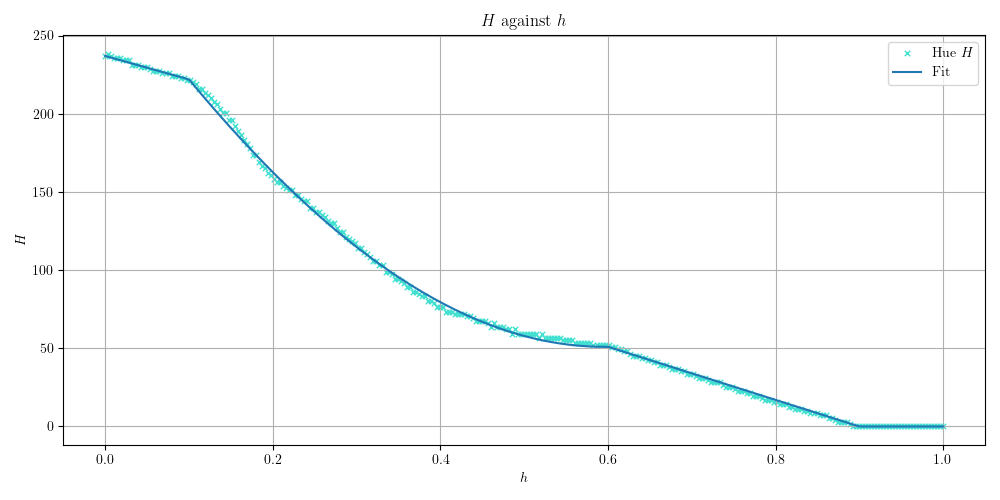
\includegraphics[scale = 0.55]{v-against-h.png}
    \caption{The fit result for \(f_V: h \mapsto V\)}
    \label{fig:v-against-h}
\end{figure}

Note that in this plot, \(V\) when \(h = 0\) or \(h = 1\) is excluded, since just like every \(h = 0.1 k\) for some \(k \in \mathbb{N}\), they are anomalies created by the horizontal black line in the scale.

To find \(f^{-1}: \mathcal{C} \to [0, 1]\), we do not need necessarily to find an expression of \(h\) in terms of \((H, V, S)\). If we notice that \(f_H\) is one-to-one on \(h \in [0, 0.9]\), and \(f_V\) is one-to-one on \(h \in [0.9, 1]\), we can use \(f_H^{-1}\) to determine \(h\) from \(H\) only if \(H\) is non-zero, and use \(f_V^{-1}\) otherwise.

\[
    f^{-1}(H, S, V) = \begin{cases}
        f_H^{-1}(H), & H \neq 0, \\
        f_V^{-1}(V), & H = 0.
    \end{cases}
\]

Notice that for \(h \in [0.1, 0.6]\), \(f_H\) is a cubic and is not easily invertible. However, it would be plausible to use a binary-search algorithm to find \(h\) based on \(H\) since it is monotonic, and it is within a reasonable amount of time, to relatively good accuracy. Otherwise, on the linear parts, it is fine to simply mathematically invert it.

\subparagraph{Flowchart of data and sidenotes} To summarise, we discussed the mapping from the colour space\(\mathcal{C}\) to the normalised height \(h\), and back, and we also discussed how \(h\) is related with the measured intensity \(I\), the PGA \(a\), the PGV \(v\), and the PGD \(x\). They can be transformed forwards and backwards using simple mathematical explicit relations, and specifically for \(f_H^{-1}(H)\) will use a binary search algorithm.

Figure \ref{fig:kmoni-data-flow} shows the data flow, Figure \ref{fig:variable-relation} shows the relation between abstract variables, and \ref{fig:generated-colour} shows the result of colour generated compared with the original.

\begin{figure}[!ht]
    \centering
    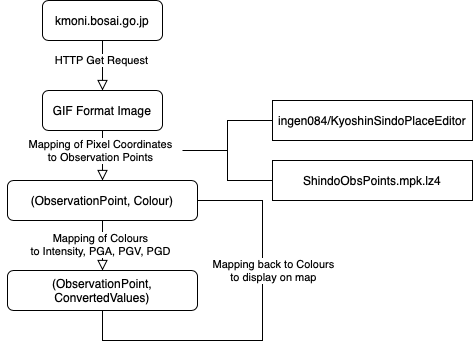
\includegraphics[width = 0.8\linewidth]{kmoni-data-flow.png}
    \caption{Flow of data in NIED data sources}
    \label{fig:kmoni-data-flow}
\end{figure}

\begin{figure}[!ht]
    \centering
    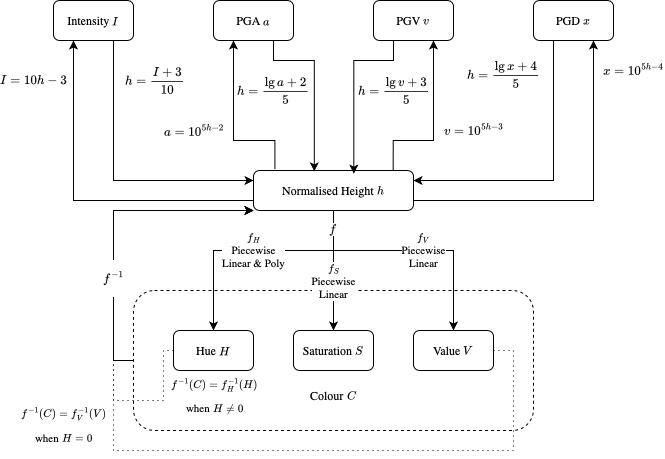
\includegraphics[width = 0.9\linewidth]{variable-relation.png}
    \caption{Relation between abstract variables}
    \label{fig:variable-relation}
\end{figure}

\begin{figure}[!ht]
    \centering
    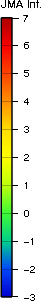
\includegraphics[scale = 0.6]{jma-scale.png}
    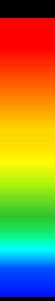
\includegraphics[scale = 0.6]{generated-colour.png}
    \caption{Colour generated using fitted functions}
    \label{fig:generated-colour}
\end{figure}

% TODO: Draw the diagram!

It is worth noting that an existing NuGet Library, \GitHubHref{ingen084}{KyoshinMonitorLib} which is designated to manage intensities, as well as extracting intensities from the 'Kyoshin' monitor. This NEA did refer to this for some guidance but is not dependent on this library, and its necessary functionalities within the scope of this NEA is realised again using the author's own code. The developer of this library did also mention that it is quite purpose-built so might not be suitable for general use.

It is also worth noting that, technically, scraping the data from the 'Kyoshin' monitor page of NIED is not explicitly allowed, but not explicitly banned either. However, extracting and displaying numerical data in the application is strictly banned by the NIED, and therefore the numerical values will only serve as internal values of the application and will not be displayed in any way.

This paragraph referred to \href{https://qiita.com/NoneType1/items/a4d2cf932e20b56ca444}{the blog article} written by NoneType1, author of JQuake.

\paragraph{DM-D.S.S. Data Source}

DM-D.S.S. is a well-structured official data source with low latency and reliable information and services. This is going to be the primary data source for most part of the application.

Their APIs are split into two types: HTTP based requests and WebSocket based connections. HTTP based requests are typically for more static information, while WebSocket connections are for live time-essential data feeds, such as the EEW warnings and latest earthquake information.

\subparagraph{Authorisation} There are two types of authorisation that DM-D.S.S. supports, API Keys and OAuth2 Access Tokens.

API Keys access tokens are extremely easy to program, since it simply uses Basic BasicBath64 Authorisation in the header, and uses the key as the username (without a password). However, this introduces an extra layer of complexity for the users, since they would have to go to the settings of the DM-D.S.S. webpage and achieve an API Key to paste into the application, as shown in Figure \ref{fig:api-key-control-panel}.

\begin{figure}[!ht]
    \centering
    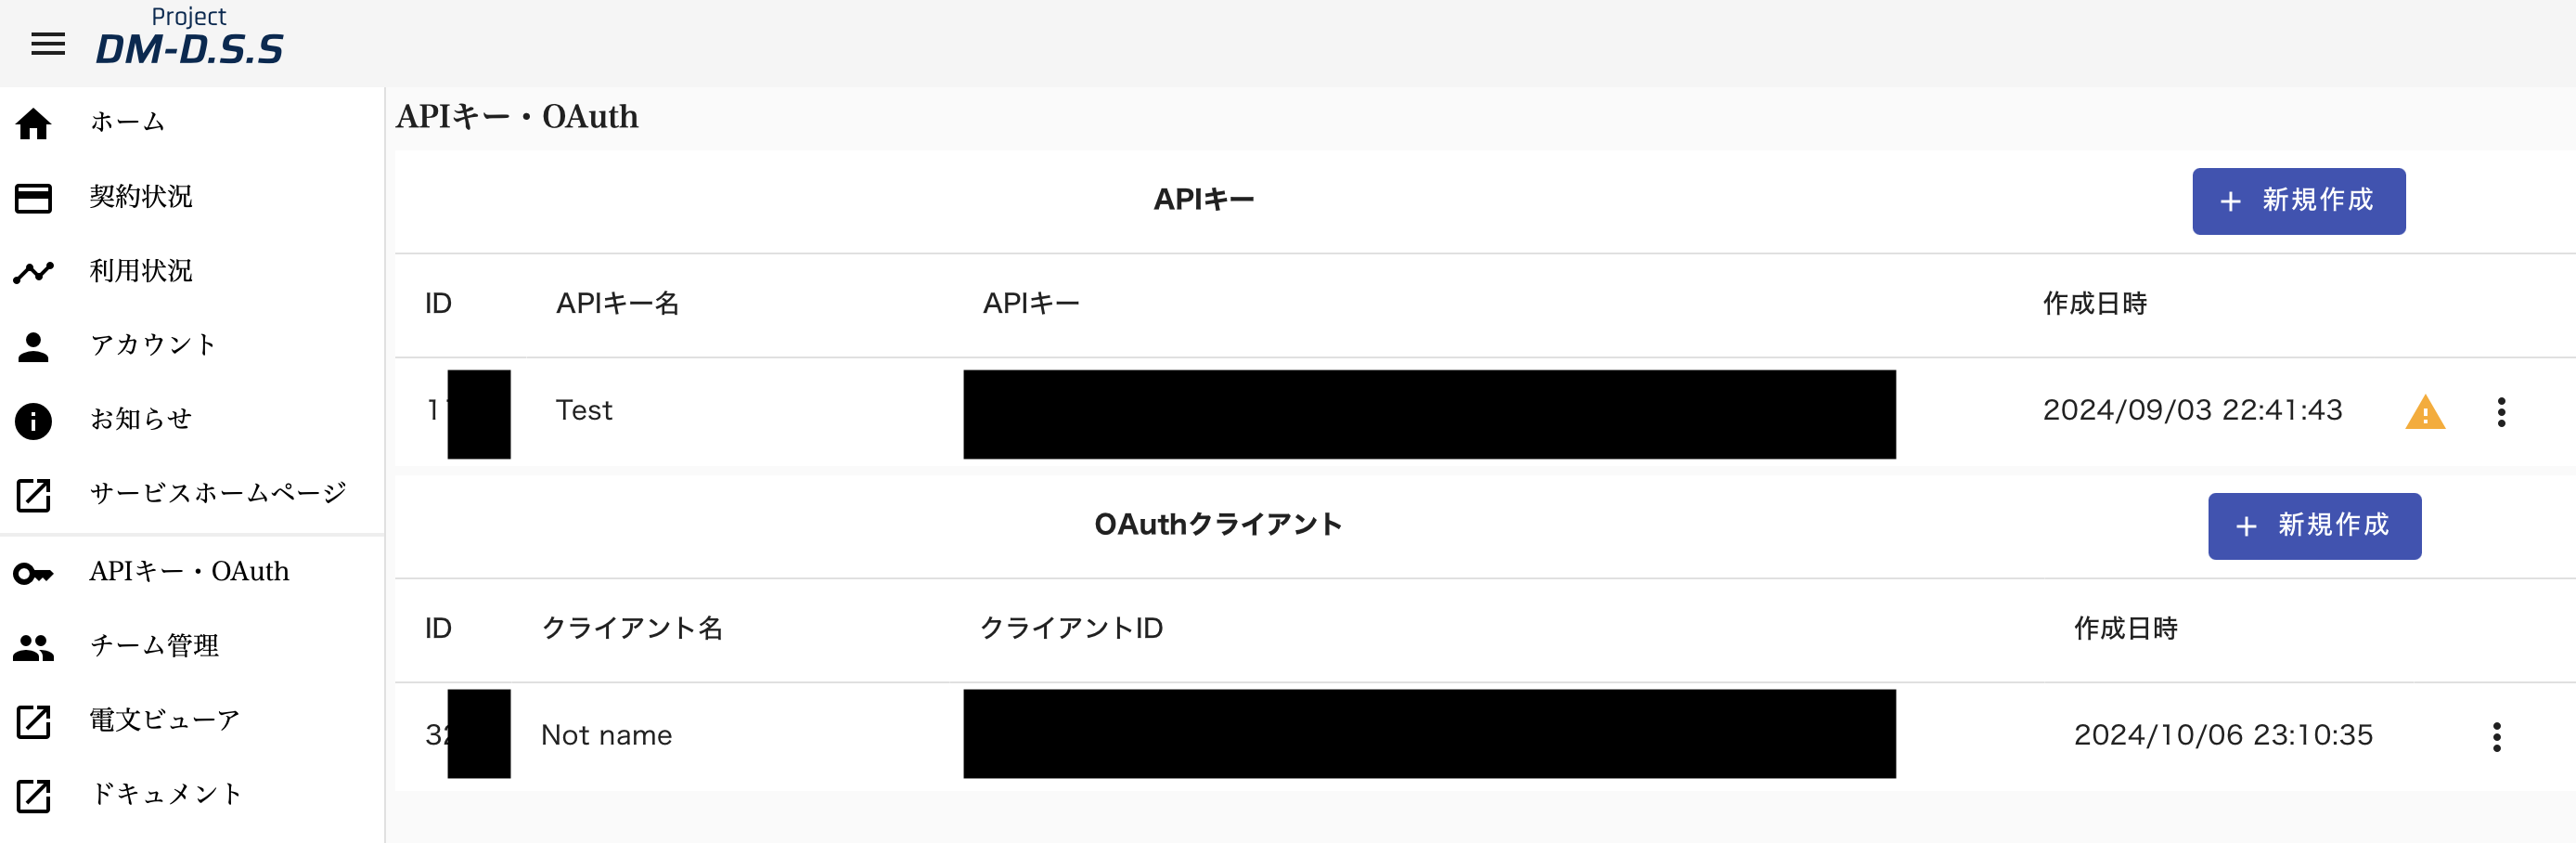
\includegraphics[width = 0.7\linewidth]{api-key-control-panel.png}
    \caption{Control panel for API Keys}
    \label{fig:api-key-control-panel}
\end{figure}

As for OAuth2, it will be much simpler for the users,

% TODO: I don't really understand how OAuth 2.0 works.

For the purposes of this NEA, we will primarily use the API Key way of accessing DM-D.S.S. since it will be easier to code and debug, and OAuth2 will introduce quite a lot of complexity to the program. However, the program should be designed to be able to modify to OAuth2 authentication without much modification, and if time permits OAuth2 will be implemented in the application.

\subparagraph{HTTP Based Requests}



\subparagraph{WebSocket Connections}

\subparagraph{Flowchart of data and sidenotes} It is worth noting that an existing NuGet Library, \GitHubHref{ingen084}{DmdataSharp} supports dealing with the DM-D.S.S. data flow and converting them to C\# objects (and exceptions). However, for the purposes of this NEA, we will implement our own way to interact with the APIs and the correlated C\# DTOs. The developer of this library did also mention that it is quite purpose-built so might not be suitable for general use.

\subsubsection{OOP Model}
OOP modelling (classes, methods, attributes, inheritance etc.). Class diagrams would be useful (these are covered in Bond book 1 page 185 onwards). Diagrams should follow conventions for inheritance/composition and private/protected/public methods/attributes.

\subsection{Hierarchy Chart}
As discussed in the analysis section, the program consists of three parts: data-parsing from external data sources, GUI functionalities and joint functionalities, where the GUI part will be divided into two parts focusing on real-time monitoring and past-earthquake information, respectively. A detailed discussion into how different modules can be further split up while at the same time being interacted is discussed, and Figure \ref{fig:hierarchy} is a hierarchy diagram for the whole application. This shows how \textbf{decomposition} technique is applied to reduce a sophisticated problem into more attackable problems.

A top-down approach to problem-solving will lead to the identification of tasks with sub-tasks. i.e. modules and functions required.

\begin{figure}[!ht]
    \centering
    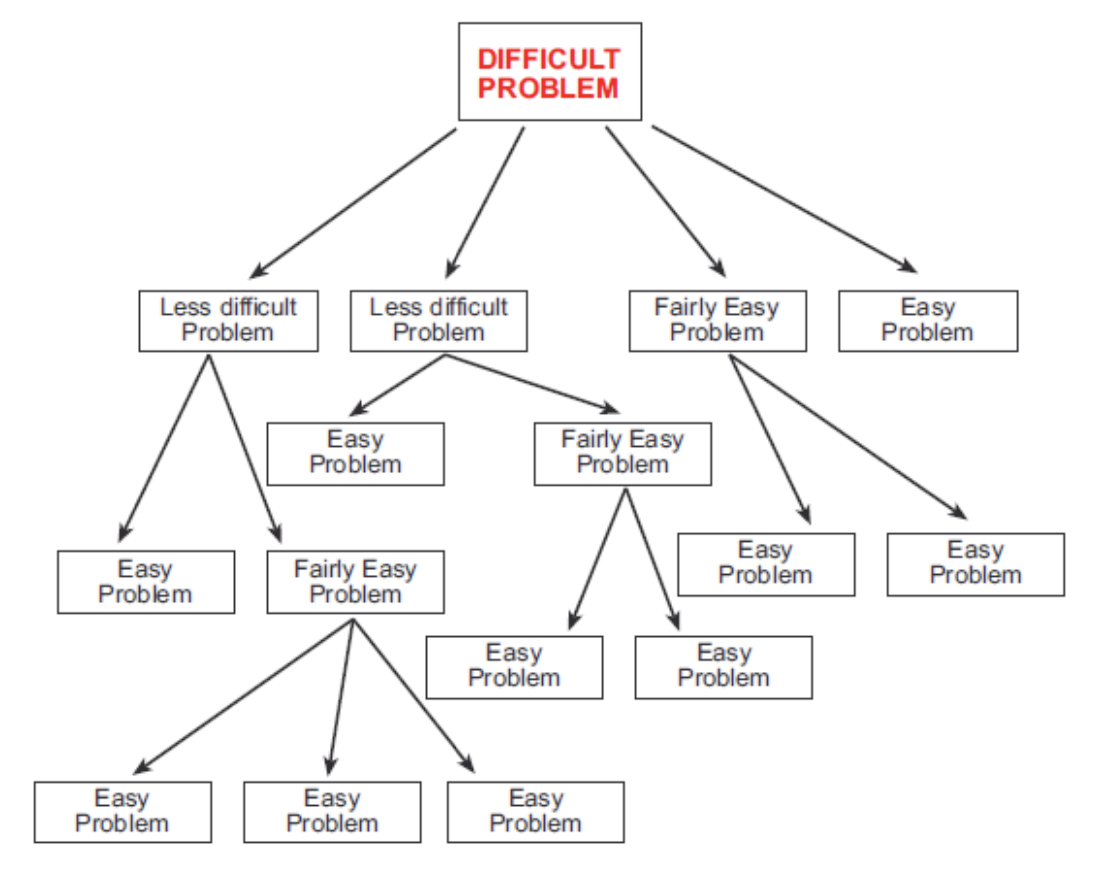
\includegraphics[width = 0.5\linewidth]{hierarchy_chart.png}
    \caption{Hierarchy Chart.}
    \label{fig:hierarchy}
\end{figure}

\begin{figure}[!ht]
    \centering
    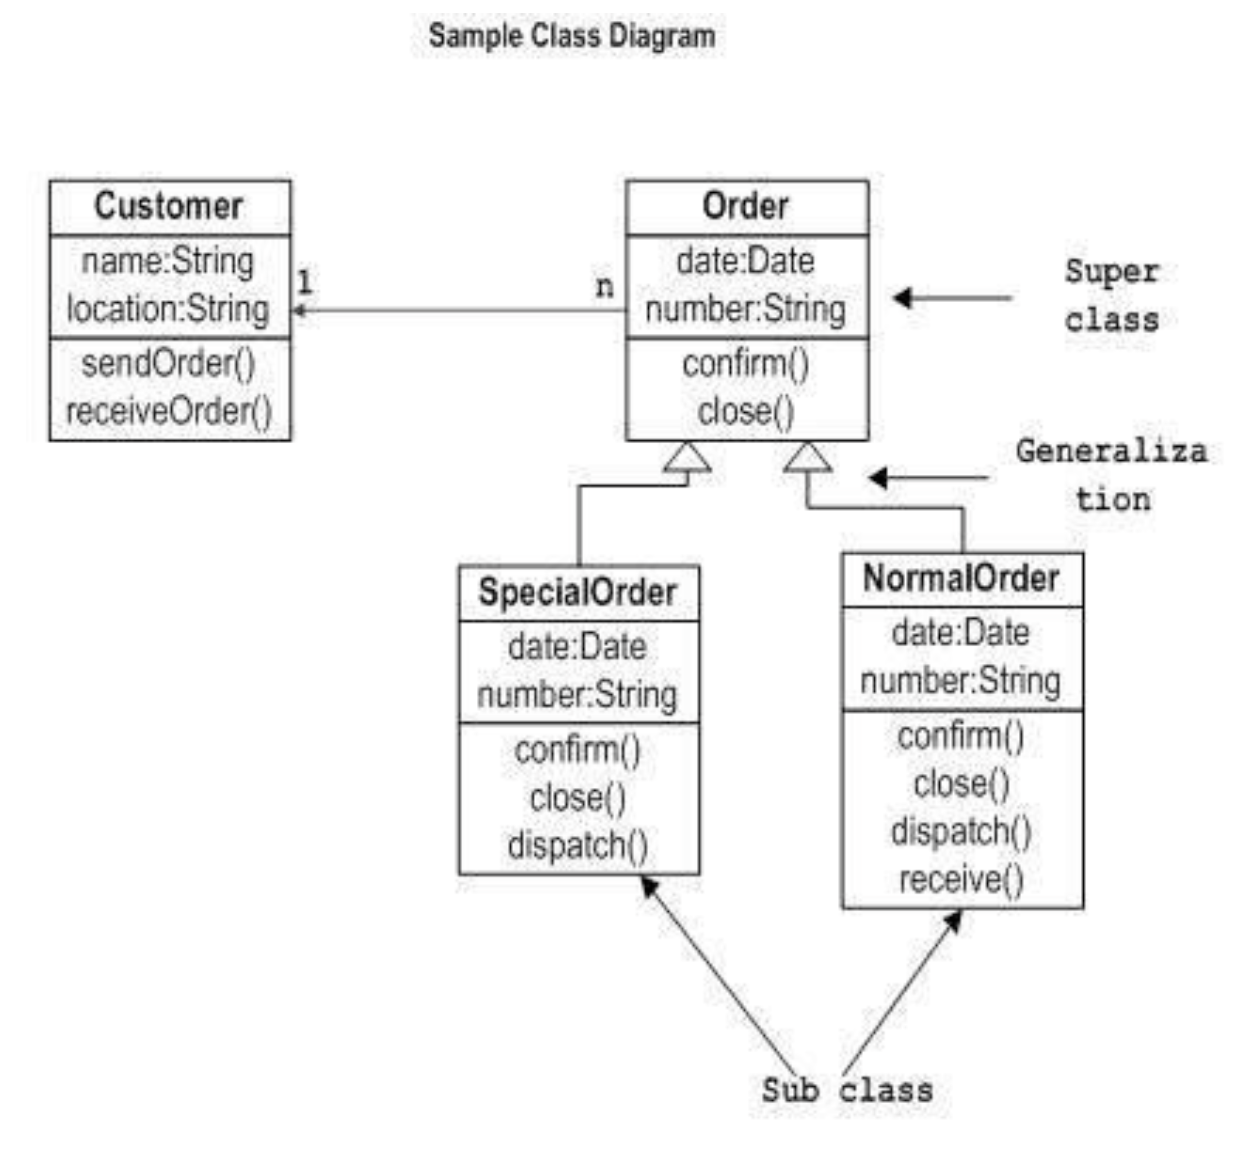
\includegraphics[width = 0.5\linewidth]{class_diagram.png}
    \caption{Class Diagram.}
    \label{fig:classes}
\end{figure}

\subsection{User Interface}
You will need to draw up a prototype for the user interface. You may do this within the software package you implement your solution in.
\begin{itemize}
    \item Screen designs
    \item Menu options/sequences
    \item Buttons/keys/commands (command line)
\end{itemize}

\subsection{Hardware \and Software Requirements}
Draw up a hardware and software specification for items that are required.

\section{Technical Implementation}
\subsection{Key Code Segments}
\subsubsection{Data structures}
Implementation of ADTs and OOP Classes to be demonstrated.

\subsubsection{Modularity}
Code should be created and tested in separate modules that are integrated later. Use subheadings for each module, define the purpose of the module, and show unit testing of the module.

\subsubsection{Defensive Programming/Robustness}
Exception handling

\section{Testing}
Consider how you will test your project. You should devise a test strategy that encompasses a range of methods.

\subsection{Test Strategy}
\begin{itemize}
    \item Unit testing (of individual functions)
    \item Integration testing (e.g. different modules/class files)
    \item Robustness (demonstrating defensive programming skills/exception handling)
    \item Requirements testing (against your initial requirements - a table with test number, description, test data, expected result, evidence (screenshot/video time link) would be suitable)
    \item Independent end user beta testing (this will assist with your evaluation)
\end{itemize}

\subsection{Testing Video}
\begin{itemize}
    \item You can include a video to assist (but you will need to reference the time point at which relevant evidence appears)
    \item If you include a video you will need to have it publicly available.
    \item It is suggested that you include a QR code in your testing to give a link to it the video (for the moderator) rather than just giving a long URL on its own.
\end{itemize}

\subsection{System Tests (against original requirements' specification)}
You need to give evidence in support of requirements that have been met e.g. reference to a relevant test/screenshot/relevant code.

\begin{table}[!ht]
    \centering

    \begin{tabular}{|l|p{0.15\linewidth}|l|p{0.3\linewidth}|}
        \hline
        Requirement \textnumero & Description & Success Criteria & Tests + Evidence \\
        \hline \hline
                                &             &                  &                  \\
        \hline
                                &             &                  &                  \\
        \hline
                                &             &                  &                  \\
        \hline
    \end{tabular}
    \caption{Table of Tests.}
    \label{table:tests}
\end{table}

\section{Evaluation}
\subsection{Requirements Specification Evaluation}
Personal evaluation
\begin{itemize}
    \item Copy and paste your original requirements from your project analysis
    \item You need to review each requirement and comment objectively on whether it was \textit{fully met/partially met/not met}.
\end{itemize}

\begin{table}[!ht]
    \centering

    \begin{tabular}{|l|p{0.15\linewidth}|l|p{0.3\linewidth}|}
        \hline
        Requirement \textnumero & Description & Success Criteria & Fully/Partial/Not met (Reflective Comment) \\
        \hline \hline
                                &             &                  &                                            \\
        \hline
                                &             &                  &                                            \\
        \hline
                                &             &                  &                                            \\
        \hline
    \end{tabular}
    \caption{Table of Evaluation.}
    \label{table:evaluation}
\end{table}

\subsection{Independent End-User Feedback}
End user/client evaluation
\begin{itemize}
    \item there \textbf{must} be meaningful end user feedback
    \item You should hold a review meeting with your end user
    \item Write down any key feedback that they give you. E.g. Agreement that a particular requirement has been meet/comments as to aspects that they find suboptimal/comments as to additions they would like to see
\end{itemize}

\begin{table}[!ht]
    \centering

    \begin{tabular}{|l|p{0.15\linewidth}|l|p{0.3\linewidth}|}
        \hline
        Requirement \textnumero & Description & Acceptance Y/N & Additional Comments \\
        \hline \hline
                                &             &                &                     \\
        \hline
                                &             &                &                     \\
        \hline
                                &             &                &                     \\
        \hline
    \end{tabular}
    \caption{Table of Feedback.}
    \label{table:feedback}
\end{table}

\subsection{Improvements}

You need to give consideration to a number of potential future improvements that could be made. They may arise from either your experience or from feedback given to you by your end user. Ideally at least one should be in response to end user feedback.

\begin{itemize}
    \item Write a paragraph for each potential improvement/change
    \item The improvements/changes could result from additional functionality that has been identified as being beneficial or could be as a result of required efficiencies if some processes are clunky or require faster run-times
    \item You should then comment on how the proposed change could be implemented moving forward. i.e. what would need to be changed/developed and how? You are not expected to actually make any changes; just comment on the possibilities.
\end{itemize}

\section{Code Listing}

\end{document}